\documentclass[]{article}
\usepackage[round]{natbib}

\usepackage{fullpage}
\usepackage{listings}
\usepackage{url}
\usepackage{authblk}
\usepackage{graphicx}
\usepackage{color}
\usepackage{booktabs}
\usepackage{amsfonts}
\usepackage{amsmath}
\usepackage{bm}
\usepackage{xspace}

\lstset{language=Python}

% cross-reference with main text
\usepackage{xr}
\externaldocument{paper}

% local definitions
\newcommand{\sgcomment}[1]{{\textcolor{red}{SG: #1}}}
\newcommand{\bmhcomment}[1]{{\textcolor{blue}{BMH: #1}}}
\newcommand{\aprcomment}[1]{{\textcolor{magenta}{APR: #1}}}
\newcommand{\tdwcomment}[1]{{\textcolor{cyan}{TDW: #1}}}

\newcommand{\E}{\mathbb{E}}
\newcommand{\moments}{\texttt{moments}\xspace}
\newcommand{\Relate}{\texttt{Relate}\xspace}
\newcommand{\msprime}{\texttt{msprime}\xspace}
\newcommand{\demes}{\texttt{demes}\xspace}

\usepackage{array}
\newcolumntype{P}[1]{>{\raggedright\arraybackslash}p{#1}}

\begin{document}
\title{Supporting Information for\\
``A weakly structured stem for human origins in Africa''}
\author{Aaron P. Ragsdale, Timothy D. Weaver, Brenna M. Henn, and Simon Gravel}
\date{\today}
\maketitle

\renewcommand{\thefigure}{S\arabic{figure}}
\renewcommand{\thetable}{S\arabic{table}}
\renewcommand{\theequation}{S\arabic{equation}}
\setcounter{figure}{0}
\setcounter{table}{0}
\setcounter{equation}{0}

\tableofcontents
\newpage

\section{Data and sequencing}

\subsection{Sequencing and variant calling}

Low coverage (4-8x) Illumina short read data were generated for the Nama,
Gumuz, Amhara and Oromo populations as part of the African Diversity Reference
Panel (Sanger / Wellcome Trust) \citep{Gurdasani2015-qy,Pagani2015-pz} and
approved through a secondary data analysis agreement for this project. Briefly,
raw reads were aligned to GRCH37 with BWAmem \aprcomment{cite}, duplicates
marked with Picard MarkDuplicates, reads were realigned around indels with GATK
RealignerTargetCreater / IndelRealigner followed by BQSR with dbSNP 137.
Contamination checks were performed requiring that FREEMIX $<0.05$;
contamination checks resulted in the elimination of 22 Nama samples. We note
that the high heterozygosity in these genomes both due to inherent genetic
diversity and admixture may have violated base assumptions for this
heterozygosity check. Genomes were then variant called with GATK3.2 Unified
Genotyper \aprcomment{cite} using joint calling across 2,478 individuals within
the ADRP dataset with a minimum base quality of 17. Data were merged with 1000
Genomes Phase 3 \citep{1000_Genomes_Project_Consortium2015-zq} using the union
of sites identified with bcftools isec (-n+1) \aprcomment{cite} then refined
with Variant Recalibrator with a truth sensitivity threshold of 99.5\%. HapMap
III and dbSNP 138 served as known sites while 1000 Genomes Phase 1 Omni2.5 and
Phase 1 genomic SNP served as the training set. After VR, no batch effects were
observed along PC1 and PC2 for 1000 Genomes vs. ADRP. Phasing on the combined
dataset was performed via SHAPEIT2 \aprcomment{cite} and utilized the duoHMM
option for duos and trios. We highlight 82 Nama genomes which are newly
available (unpublished) under accession number EGAD00001006198. Among these 82
Nama samples, we down-sampled the individuals to minimize close relatives and
admixture, such that 44 Nama genomes were retained. 2nd and 3rd degrees
relatives were inferred from reconstructed pedigrees with Omni2.5 SNP array
data. Individuals with $>70\%$ estimated Khoe-San ancestry were retained for
analysis, after partitioning ancestry into $k=6$ clusters with ADMIXTURE
\aprcomment{cite} where alternative ancestries represent European, West
African, Near Eastern, and East African gene flow. 

\subsection{Nama sample collection and consent}

DNA samples were collected from three Nama communities in the Richtersveld
region of South Africa, which borders southern Namibia, in 2012. A community
guide was present during each interview and facilitated consent in Afrikaans or
Nama. Written consent was recorded per our IRB protocol with human subjects
approval from Stanford University (Protocol \#13829), Stellenbosch University
(N11/07/210) and later maintained via SUNY Stony Brook (Protocol \#727494).
Saliva samples were extracted from Oragene [OGR-500] kits at Stellenbosch
University. Results stemming from genetic analyses have been communicated in
2015, 2019, 2021 via community presentations, a radio interview and to
representatives of the Richtersveld National Park.

\subsection{Details about populations used in analyses}

\sgcomment{To be expanded. TODO: Brenna}
\begin{itemize}
    \item From the merged dataset of the African Diversity Reference Panel and
        1000 Genomes phase 3 data, subsampled to population included in this study
    \item West Africa: Mende from Sierra Leone (MSL); South Africa: newly sequenced 
        Nama; East Africa: Gumuz (traditionally hunter-gatherer with low levels of 
        Eurasian admixture), Oromo and Amhara (combined as traditionally 
        agriculturalists with large proportion of back-to-Africa Eurasian ancestry); 
        Eurasian: British (GBR)
    \item Combined with the high coverage Vindija neanderthal genome
    \item For running \Relate, we used a larger set of populations. We kept all 
        African 1000 Genomes populations, along with the Nama, Gumuz, Oromo, and
        Amhara, as well as 4 Eurasian populations from 1000 Genomes: GBR, CEU, PJL,
        and CHB
\end{itemize}

\subsection{Filtering and subsetting data}

All analyses presented in this work focus on biallelic single nucleotide
polymorphisms within the 1000 Genomes Phase 3 strict mask.  For the
\moments-LD analysis, we focused on intergenic regions because these
appear less affected by natural selection compared to both synonymous and
nonsynonymous variation \citep{Ragsdale2018-dd}. To enable comparison with
Neanderthal DNA, we excluded regions for which the Vindija Neanderthal sample
had less than 100 contiguous base pairs. 

\section{Computing statistics}

\subsection{LD and diversity statistics used in model fits}
\label{sec:supp-ld-stats}

We used multi-population linkage disequilibrium (LD) and pairwise diverisity
statistics to fit demographic models to data. These statistics, introduced and
described in detail in \citet{Ragsdale2019-nt}, are the multi-population analog
of the classic LD statistics first described and computed by
\citet{Hill1968-vu,Ohta1971-yd}.

Given two biallelic loci, with alleles $A$ and $a$ and the left locus and
allels $B$ and $b$ at the right locus, the standard covariance measure of LD is
$D=p_{AB}p_{ab}-p_{Ab}p_{aB}$, where $p_{AB}$ is the frequency of $AB$
haplotypes in a population (and thus the probability of drawing an $AB$
haplotype in a random sample of that population). \citet{Hill1968-vu} solve for
the expectation of $D^2$ using a system of equations that includes $\E[Dz] =
\E[D(1-2p_A)(1-2p_B)]$ and $\E[\pi_2] = \E[p_A(1-p_A)p_B(1-p_B)]$, where $p_A$
and $p_B$ are the frequencies of $A$ and $B$ at the left and right loci,
respectively. This system also requires the expected pairwise diversity (or
expected heterozygosity, assuming random mating), denoted $\E[H] =
\E[2p_A(1-p_A)] = \E[2p_B(1-pB)]$, assuming equal mutation rates at the two
loci.

\citet{Ragsdale2019-nt} showed how to compute the analogous multi-population
set of LD statistics, and we refer readers there for details on their
definitions, computation, and interpretations. In short, we obtain expectations
of $D^2$ in each population, the cross-population product $D_iD_j$ (where $i$
and $j$ index populations), as well as those additional statistics $Dz$ and
$\pi_2$ taken over different combinations of population indexing. That is
$Dz_{i, j, k} = D_i(1-2p_{A,j})(1-2p_{B,k})$ and
$\pi_{2;i,j,k,l}=p_{A,i}(1-p_{A,j})p_{B,k}(1-2p_{B,l})$. We consider statistics
normalized by $\pi_2$ in a reference population (throughout, we use the Mende
$\pi_2$), which removes any dependence on the mutation rate. Thus, statistics
take the form $\sigma_{d;i,j}^2 = \frac{\E[D^2_{i,j}]}{\E[\pi_2]}$,
$\sigma_{Dz;i,j,k}=\frac{\E[Dz_{i,j,k}]}{\E[\pi_2]}$, and so on.
Multi-population pairwise diversity statistics $\E[H_i]=\E[2p_i(1-p_i)]$ and
$\E[H_{i,j}] = \E[p_i(1-p_j) + p_j(1-p_i)]$ were also normalized by $H$ in the
Mende, so that all pairwise diversity measures are relative to the reference
population.

$\sigma_{Dz}$ has been shown to be sensitive to deep population structure and
archaic admixture \citep{Ragsdale2019-nt}, and this statistic is closely
related to $S^*$ statistics used to scan for introgressed haplotypes
\citep{Plagnol2006-lt}. Pairwise diversity statistics $H_{i,j}$ have also been
widely used in demographic inference involving ancient DNA and many samples, as
$f_2$, $f_3$ and $f_4$ statistics can be expressed as linear combinations of
$H_{i,j}$. $f$-statistics form the basis of admixture graph analysis
\aprcomment{cite}. Therefore, the set of statistics used here encompass
multiple features of genetic data that have been used to infer models of
archaic admixture and population structure involving many populations.

\aprcomment{We used the Omni YRI map (though see figure showing similarity to
statistics under the HapMapII map). Assumed a generation time of 29 years for
rescaling times in years to generations.}

\subsection{Computing LD and diversity statistics}\label{sec:computing-stats}

We compared single- and two-locus statistics in the data to predictions based
on detailed demographic models. Model predictions were obtained using
recursions described in \citet{Ragsdale2019-nt} and implemented in the software
\moments (\url{https://bitbucket.org/simongravel/moments/src/main/}).
The model computes expected patterns of single-nucleotide pairwise diversity
and linkage disequilibrium as a function of recombination distance between
variants within and across populations, under the assumption of neutrality.

For numerical convenience, observed genetic variants were binned by
recombination distances. We assessed the robustness of the statistics to errors
in the recombination maps by considering two different recombination maps, the
OMNI YRI and HapMapII
\citep{1000_Genomes_Project_Consortium2015-zq,International_HapMap_Consortium2007-vn}.
Statistics were largely unchanged by using a different map
(Figure~\ref{fig:supp-omni-hapmap-comparison}). \aprcomment{These maps are both
inferred using array data, which is sparse. Comment on this.}

We removed bins of recombination distance less than a recombination distance of
$r = 5\times10^{-6}$ (at a rough estimate of 1 cM/Mb, this corresponds to a minimum
distance of 500 bp on average) to avoid previously reported biases at short
distances due to processes like multinucleotide mutations
\citep{Harris2014-zg,Ragsdale2019-nt}. To avoid uncertainty in phasing, we used
unphased genotypes to compute LD statistics, as proposed in
\citet{Ragsdale2020-nz}. 

Finally, we estimated uncertainty due to the finite amount of genetic material
used in inference using bootstrap over 500 segments along the genome with
roughly equal lengths of retained sequences within each segment. First, for
each distance bin, we used these bootstrap samples to obtain a
variance-covariances matrix across all statistics. This variance-covariance
matrix was used to obtain a model likelihood for each recombination distance
bin and single-locus nucleotide diversity, as a multivariate Gaussian
likelihood. The full model likelihood was taken as the product of likelihoods
over each bin. In other words, we optimized a composite likelihood where
observations in different bins were taken to be independent. To account for
correlations across bins in uncertainty estimates, we estimated parameter
confidence intervals using the same bootstrap set using the Godambe information
matrix \citep{Coffman2016-yq}. \sgcomment{is redundancy here with section
"Optimization using moments". I think we can get rid of this and say:
"optimization and uncertainty calculations are described in section
"Optimization using moments""?, This may be a bit more complicated, since the
Optimizatino section relies on this description. I think we should just punt
the bootstrap description to that section. TODO: discuss Aaron + Simon}

\subsection{Estimating two-locus statistics with small sample sizes}

The approach from \citet{Ragsdale2020-nz} provides unbiased estimates of the LD
statistics considered here, which can be directly compared to expectations for
those same statistics computed from the multi-population Hill-Robertson system.
Estimated statistics for populations with smaller sample sizes have greater
uncertainty, which is accounted for by computing variances and covariances via
bootstrap over genomic regions, assuming that there is no correlation between
distant genomic regions (i.e., no long-range LD).

Some statistics, such as $\E[D_i D_j]$, require at least two diploid samples
from a population to compute. Since we used a single Neanderthal sample, such
statistics for the Neandertal population were not used in the fit. By contrast,
there are statistics that only require a single sample in a given population to
estimate. These include cross-population nucleotide diversity measures, as well
as some LD statistics involving more than one population. For example,
statistics of the form $D_{human}(1-2p_{human})(1-2q_{neanderthal})$ require a
single Neanderthal sample and are informative of the Neanderthal demography.
These statistics were included in the fit, but statistics requiring more than
one Neanderthal sample to estimate were removed.

\subsection{Computing conditional SFS}\label{sec:computing-csfs}

The conditional site frequency spectrum (or cSFS) is the distribution of allele
frequencies restricted to loci that satisfy a given condition. Specifically, we
consider the distribution of allele frequencies in present-day populations
conditioned on the Vindija Neanderthal carrying the derived allele relative to
the inferred ancestral allele. Ancestral alleles alleles were determined from a
6 primate alignment \aprcomment{cite}. This cSFS is expected to be close to
uniform under neutrality and a simple split model (with no subsequent
migration) between the ancestors of modern humans and Neanderthal
\citep{Chen2007-iy}. By contrast, a U-shaped distribution has been taken as
evidence for archaic introgression from a population whose split from modern
humans is at least as old as that of the human-Neanderthal split
\citet{Durvasula2020-td,Yang2012-ze}. Because we wanted to compare our
inferences (based on intergenic sites) to inferences from previous work (based
on whole-genome data), we computed the cSFS for both intergenic and all sites
genome-wide. Sites with no calls in the Vindija Neanderthal were excluded from
this analysis. \aprcomment{Figures XX.}

Because we were concerned that cSFS analyses may be affected by incorrect
inference of the ancestral allele \cite{Hernandez2007-mf}, we computed the cSFS
for all mutations, and for transitions and transversions separately
\aprcomment{(Figure X, cSFS)}. Comparisons of these observed cSFS with model
predictions are discussed in the model prediction section below. 

\section{Model specification and fitting}

For the early history, we tested model parameterizations that cover many of the
proposed scenarios of population structure, size changes, and/or archaic
admixture. The simplest model, in terms of number of parameters, was a
single-origin expansion of modern humans, with no structure in the stem and no
archaic admixture aside from the Neanderthal admixture in Eurasian populations
following the out-of-Africa migration. This model allowed for a population size
change in the stem of modern humans between the ancestral split of the
human-Neanderthal lineages and the more recent split of branches leading to
Southern and West/Eastern African populations.

To include population structure in early human history, we considered multiple
parameterizations of models that allowed more than a single stem population. In
general, stem populations were allowed to vary in their sizes, split times, and
migration rates, with parameterizations flexible enough to encompass proposed
scenarios of either archaic admixture or population structure, both connected
by gene flow or with isolation between stems.

In one parameterization of early structure, which we refer to as a “continuous
migration” model, a secondary stem population (stem 2) split from the primary
stem (stem 1) that leads to modern humans. Stem 1 contributed to present-day
populations via a series of population splits similar to the single-origin
model, while stem 2 contributed through continuous symmetric migrations with
contemporaneous populations. The symmetrical migration rates could differ
across population pairs and over different epochs. This continuous migration
was allowed until stem 2 disappeared, which occurred as recently as 5kya. We
tested models that both allowed or disallowed migration between stems, i.e.,
before stem 1 split into S/E/W African populations.

In another parameterization of early structure, a secondary stem population
(stem 2) contributed ancestry to present-day populations via a series of
instantaneous admixture events (i.e., pulse admixture or “merger” events) to
lineages leading to sampled present-day African populations. Merger events were
allowed to occur in one or more of the Nama, Mende, and Gumuz branches, as well
as the branch of East and West Africans prior to their split. Those admixture
events were allowed to occur at any time along those branches, and with any
proportions, and stem 2 was allowed to split from the primary stem at any time
before subsequent divergences (and either before or after the split of the
Neanderthal branch). We tested models that allowed migration between the early
stems, before subsequent splits and admixture events, as well as models that
were restricted to isolation between stem branches. Depending on the specific
parameters, such models encompass commonly-considered ghost archaic admixture
scenarios (e.g., if a long-isolated lineage more recently contributes a
minority of ancestry to one or more populations), as well as relatively simple
fragmentation-coalescence scenarios.

Based on the geographical locations of present-day populations, we tentatively
labeled ancestral branches using a parsimony in migration, referring to South,
East, and West African branches (S/E/W AFR, Figure X). We do not know the
geographical location of these ancestral populations (nor even if they
correspond to populations with a well-defined geographic range), and these
labels should be considered as tentative. However, we found it useful to name
branches in reference to where in Africa their descendants are found.
\sgcomment{Please double-check this paragraph! TODO Brenna?}

\subsection{General strategy for building models and introducing complexity}

With up to six sampled populations in final demographic models that we fit,
there are many parameters to learn. Even in the simplest model involving all
populations (such as the tree-like single-origin model), there are a few dozen
parameters defining split times, migration rates, admixture timings and
proportions, and population sizes and size changes. Thus, parameter space for a
given model topology is large. In addition, the space of possible model
topologies is itself large – as the number of populations increases, the number
of possible topologies also increases, as there are more possibilities for the
order of divergence and admixture events. 

In order to narrow the set of possible models to plausible scenarios and to
avoid overfitting, we took an approach that combined the incremental addition
of complexity, starting with fewer populations before combining all
populations, as well as fixing parameters that have been previously estimated
or that fit consistently across all model scenarios. By initially considering
sets of two or three populations, we were able to narrow down the relative
orders of divergences between African and Eurasian populations. Assuming simple
isolation-with-migration models, the Nama appeared to be the earliest diverging
population of those we considered, with West African (Mende) and East African
(Gumuz) populations diverging more recently, followed by the split of the
Eurasian branch from the East African branch.

We performed an initial round of optimization including all six populations
with a family of models including single- and multiple-stem scenarios as
described in the previous section. We identified parameters that reached
consistent values across all models. These included the timings of recent or
non-central divergences and admixture events:
\begin{itemize}
    \item East/West African population split: 60ka
    \item East African/European split: 50 ka
    \item Neanderthal introgression to Eurasian branch: 45 ka
    \item Neanderthal/human split: 550 ka
    \item Eurasian back-to-African migration: 12 ka
\end{itemize}
When testing multiple variations of the more complex models, we kept these
values fixed. This reduced the potential for overfitting the more complex
models, while reducing the computational cost of optimization.

Our models also included recent events to account for known migrations,
admixtures, and growths and declines in effective population sizes. Many of
these parameters were fixed based on previous historical, genetic, or
anthropological research, namely
\begin{itemize}
    \item East African pastoralist to South African admixture: 2 ka \cite{}
    \item European to South African admixture: 10 generations ago \cite{}
    \item Mende population expansion and Gumuz population decline: 5 ka \cite{}
    \item South African population decline following colonial admixture: 9 generations ago \cite{}
\end{itemize}
While the dates of these events were fixed, the sizes and proportions were
allowed to vary in the fits. The total number of parameters that were
ultimately inferred were 18-26 \aprcomment{check!}, depending on the complexity
of the model.


\subsection{Optimization using moments}

\moments-LD uses a composite likelihood approach to simultaneously fit relative
pairwise diversity and LD statistics over a range of recombination distances.
Likelihoods were computed independently for pairwise diversity and each
recombination distance bin using a multivariate Guassian likelihood function as
described in Section \ref{sec:computing-stats}. These were multiplied across
bins and the single set of heterozygosity statistics following the approach
detailed in \citet{Ragsdale2019-nt}. For each model tested, we ran multiple
rounds of optimization, alternating between the \emph{optimize\_log\_fim},
\emph{optimize\_log\_powell}, and \emph{optimize\_lbfgsb} methods to explore
parameter space and hone in on the best fit parameters. Initial guesses for
parameters were chosen from demographically plausible starting points and then
perturbed to explore space, using gradient descent (on the log of the
parameters). The best fits from these initial rounds of optimization were then
chosen as the starting points for optimization using the Powell and/or the
L-BFGS-B methods (as implemented in the SciPy optimization package
\cite{Virtanen2020-kr}). This process was repeated with alternating
optimization methods until the best fit parameter set converged consistently.

\subsection{Confidence intervals using Godambe methods}

The bootstrap replicates that were used to compute the variance-covariance
structure of the observed statistics within bins were also used to build 500
bootstrap replicates of the data by resampling with replacement. For the best
fit parameters, we computed confidence intervals using the Godambe Information
approach, which corrects composite likelihood estimates of confidence intervals
to account for nonindependence in the data, including linkages between loci and
nonindependence of recombination bins \cite{Coffman2016-yq}.

Tables~\ref{tab:supp-single-origin}--\ref{tab:supp-merger-with-stem-migration}
give the best fit values for all parameters in the four models considered here,
along with standard errors using computed using the Godambe method.
Figures~\ref{fig:supp-single-origin-fits}--\ref{fig:supp-merger-with-stem-migration-fits}
show the corresponding fits to many of the LD statistics used in the inference.
The $\sigma_{Dz}$ statistics are fit poorly by the single-origin model, while
the models with multiple stems all provide reasonable fits to the data. The
merger-with-stem-migration model performed the best of these four models,
although the fits were nearly visually indistiguishable from the fits from the
merger-with-stem-migration model.

\section{Gene genealogy reconstruction}
\label{sec:relate}

We used \Relate version 1.0.16 \citep{Speidel2019-nj} to reconstruct genome-wide
gene genealogies using a combined set of 1000 Genomes and African Diversity
Reference Panel datasets, retaining all AFR-labeled populations and GBR, CEU,
PJL, and CHB from the 1000 Genomes panel and the Nama, Gumuz, Oromo, and Amhara
from ADRP. We used all autosomes and applied the 1000 Genomes Phase 3 strict
mask, we used an ancestral sequence determined by a 6-primate alignment
(human\_ancestor\_GRCh37\_e59), and we used the HapMap II combined
recombination map, all in GRCh37 coordinates. We assumed a generation time of
29 years, a mutation rate of 1.25e-8, and followed the standard pipeline
described in the \Relate documentation.

From the reconstructed gene genealogies, we computed coalescence rates within
and between populations using \Relate’s function \texttt{RelateCoalescentRate}.
This allows for an estimate of the instantaneous inverse coalescence rate
(IICR) for samples drawn within each population (the inverse of which is often
interpreted as the effective population size history), and the relative cross
coalescence rates between pairs of populations (which are commonly used to
estimate divergence times).

Following \citet{Speidel2019-nj} we also identified “deep branches” within gene
trees. Such a “deep branch” is a branch within a marginal tree (meaning, the
tree at a given locus) that has its upper end (i.e., the node of its
coalescence with another branch) extending to more than 1 million years in age,
and we partitioned deep branches based on their lower node ages (where two or
more branches coalesce into this single branch) into bins between 0 and 1Ma.
Such branches can be categorized by their association with Neanderthals by
comparing mutations that fall upon such a branch to the allele found in a
Neanderthal genome sequence. For this, we used the published high-coverage
Vindija Neanderthal \citep{Prufer2017-kk}. Again following the analysis in
\citet{Speidel2019-nj}, if one or more mutations on a deep branch (carrying at
least two derived mutations) are shared with the Neanderthal sequence, the
branch is inferred to have passed through the Neanderthal lineage.

A deep branch is assigned to a contemporary population if at least one sample
from that population has ancestry that passes through that branch.
\citet{Speidel2019-nj} show that deep branches with lower ends more recent than
the Neanderthal introgression event are enriched for Neanderthal-matching
alleles in Eurasian populations, while a large majority of deep branches in
1000 Genomes West African populations do not match either the Neanderthal or
Denisovan samples. This observation was taken as further evidence for deep
population structure or archaic admixture in West African populations from an
unidentified hominin unrelated to the Neanderthal/Denisovan complex.

\section{Predictions from inferred demographic models}

\subsection{Divergence between coexisting populations over time}

We considered a few different measures of differentiation between populations
in four inferred models, starting with $F_{ST}.$ For each of the four inferred
demographic models presented here, we computed predicted $F_{ST}$ for pairs of
contemporaneous populations over time. 

$F_{ST}$ represents the proportion of genetic variance in a multi-population
sample that can be attributed to drift between populations in that sample
(e.g., \cite{Bhatia2013-sq}).  $F_{ST}$ depends on population divergence times,
gene flow, and population sizes. For present-day sampled populations, predicted
$F_{ST}$ can be compared to data (Fig.~\ref{fig:supp-FST-panels}), while past
estimates represent model predictions about the differentiation between past
populations. We computed $F_{ST}$ as a ratio of expected (or average)
variances, using observed pairwise diversity within and between populations as
in \citet{Peter2016-ys}:
\begin{equation}
    F_{ST}(i, j) = \frac{\E[2H_{i,j} - H_i - H_j]}{\E[2H_{i,j} + H_i + H_j]},
    \label{eq:FST}
\end{equation}

where $H_{ij}$ is the average number of differences between one haploid copy of
the genome from population $i$ and one from population $j$, and $H_i$ and $H_j$
are the average number of differences for two haploid copies from the same
population. In all inferred models, $F_{ST}$s between Neanderthals and the
ancestors of modern humans were much larger than between any pair of modern
human populations or their ancestors (stems). $F_{ST}$ between modern human
populations over the last $100ka$ remained relatively low, at $\sim0.1$ or
less. In the continuous-migration model, the two stem populations also were
predicted to have low $F_{ST}$ within this range, as migration rates were
inferred to be high enough to maintain genetic similarity. In both the
merger-without-stem-migration and the merger-with-stem-migration, one of the
stem populations was inferred to have a short, severe bottleneck, which led to
increased $F_{ST}$ between stem populations during that time. In the merger
with stem migration, $F_{ST}$ reached a maximum value of $0.3$ between stems,
intermediate between human-Neanderthal divergence ($0.54$ \sgcomment{check})
and the maximum $F_{ST}$ observed between contemporary human populations
($0.07$.) 

Whereas the high $F_{ST}$ value between Neanderthal and humans reflects both
elevated genetic differences between the genomes of modern humans and
neanderthal and reduced diversity within the Neanderthal population
(Fig.~\ref{fig:supp-FST-panels}), the increased $F_{ST}$ between the stems is
primarily due to an inferred bottleneck reducing stem diversity, while genetic
differentiation between individuals from the two stems is within the range of
genetic differentiation between (and even within) human populations. In other
words, our best fit model describes two stems with one stems showing reduced
diversity, but individuals across stems showing no more differentiation than
two modern population. \sgcomment{Previous paragraph could use rereading.}


\subsection{\bm{$f_4$} statistics between pairs of contemporary
and pairs of ancient populations}
\label{sec:f4}

To evaluate the degree to which divergence among modern populations is
inherited from divergence between early stem population, we computed f4
statistics of the form
\begin{equation}
    f_4(\text{stem}_1, \text{stem}_2; \text{modern}_1, \text{modern}_2) = 
    \E[(f_{\text{stem}_1} - f_{\text{stem}_2})(f_{\text{modern}_1}-f_{\text{modern}_2})]
    \label{eq:f4}
\end{equation}
This statistic measures co-linearity of genetic drift between modern
populations $(f_{\text{modern}_1}-f_{\text{modern}_2})$ and stem populations
$(f_{\text{stem}_1}-f_{\text{stem}_2})$ (see
Figures~\ref{fig:supp-f4s-single-origin}--\ref{fig:supp-f4s-merger-with-stem-migration}
and \citet{Lipson2020-cq}).

To contrast these statistics to divergence across modern populations,
\begin{equation}
    f_2(\text{modern}_1, \text{modern}_2) =
    \E[(f_{\text{modern}_1}-f_{\text{modern}_2})^2]),
\end{equation}
we interpret the $f$-statistics as scalar products between vectors in 
allele frequency space. In particular, the vector 
$v=(f_{\text{modern}_1}-f_{\text{modern}_2})$, 
representing differences in allele frequencies across modern populations,
can be written as $v=v_\perp + v_\parallel$, a component perpendicular and
a component parallel to the divergence $(f_{\text{stem}_1}-f_{\text{stem}_2})$
across stems. We can then decompose 
$f_2(\text{modern}_1,\text{modern}_2) = v_\perp^2+v_\parallel^2$, with  
\begin{equation}
    v_\perp^2 = f_4^2(\text{stem}_1, \text{stem}_2; 
    \text{modern}_1, \text{modern}_2)/f_2(\text{stem}_1, \text{stem}_2)
\end{equation}

Finally, the proportion of modern-day structure
$f_2(\text{modern}_1, \text{modern}_2)$ that is accounted for by the
component parallel to ancient population structure is
\begin{equation}
    \alpha^2 = \frac{v_\perp^2}{f_2(\text{modern}_1, \text{modern}_2)} =
    \frac{f_4^2(\text{stem}_1, \text{stem}_2; \text{modern}_1, \text{modern}_2)}
    {f_2(\text{stem}_1,\text{stem}_2)f_2(\text{modern}_1, \text{modern}_2)}.
\end{equation}
$\alpha^2$ can be interpreted as the proportion of the $f_2$
divergence across modern populations that is aligned with the differences in
allele frequencies across ancient populations. However, drift occurring after
the time of sampling of ancient populations is not correlated to drift
occurring before that time. For this reason, we also interpret $\alpha^2$ as the
proportion of the $f_2$ divergence across modern populations that is explained by
the differences in allele frequencies across ancient populations. We report
this predicted statistic for each of the four inferred demographic models in
Figures~\ref{fig:supp-f4s-single-origin}--\ref{fig:supp-f4s-merger-with-stem-migration}.

\begin{figure}[ht]
    \centering
    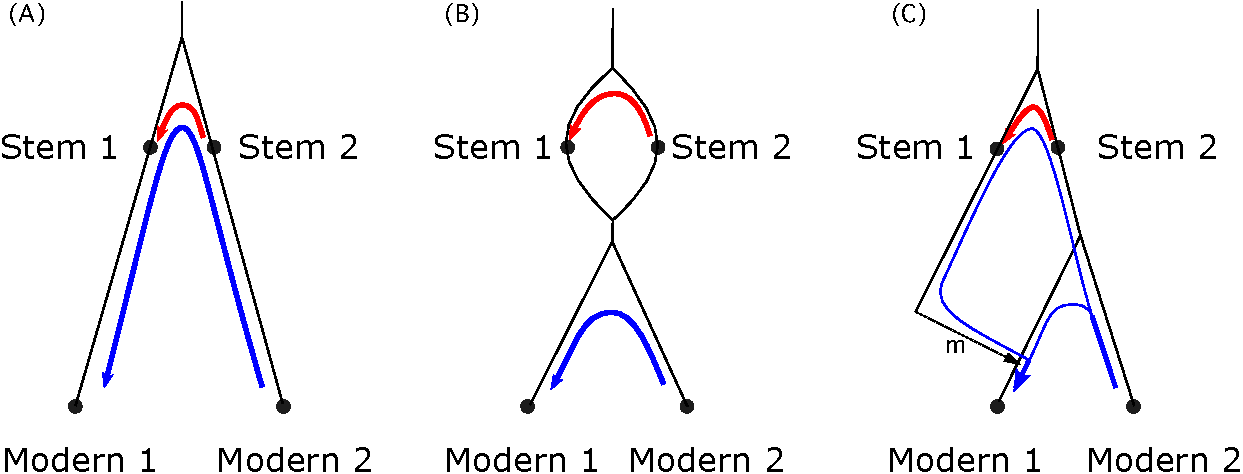
\includegraphics[width=0.75\textwidth]{figures/supp-f4-scenarios}
    \caption{
        \textbf{Present day structure attributable to ancient population structure.}
        The statistic 
        $f_4(\text{stem}_1, \text{stem}_2; \text{modern}_1, \text{modern}_2)$
        captures how much of present-day population structure can be attributed to 
        population structure among the stems. The blue line represents genetic drift 
        along ancestral branches between modern populations, while the red line 
        represents drift between stem populations. $f_4$ measures the overlap 
        between the blue and red line, which corresponds to shared genetic drift 
        between the two pairs. 
        In scenario A, modern populations are descended from distinct stems, and 
        $f_4(\text{stem}_1, \text{stem}_2; \text{modern}_1, \text{modern}_2)$
        equals the drift between stems, $f_2(\text{stem}_1, \text{stem}_2)$.
        In scenario B, despite deep population structure, there is no shared drift
        and $f_4=0$. That is, present-day population structure is unrelated to
        structure among stems. In more realistic scenario C, where $\text{modern}_1$
        receives a proportion $m$ of its ancestry from the dotted arrow, the overlap
        is only found along the corresponding path, and $f_4$ depends on both
        ancestry proportion $m$ and drift between stems,
        $f_4(\text{stem}_1, \text{stem}_2; \text{modern}_1, \text{modern}_2)
        = mf_2(\text{stem}_1, \text{stem}_2)$
        \aprcomment{Get better resolution image from Simon}
    }
    \label{fig:supp-f4-scenarios}
\end{figure}

\section{Validations using simulations from inferred demographic models}

Here we focus on four parameterizations of early human history: (1) a “single
origin” with recent expansion, (2) primary and second stem populations with
“continuous migration”, (3) two stem populations that do not exchange migrants
before merging to form regional African populations, referred to as a “merger
without stem migration”, and (4) two stem populations that are allowed to
exchange migrants before merging to form regional African populations, referred
to as a “merger with stem migration”. Given the best fit parameters for each
model
(Tables~\ref{tab:supp-single-origin}--\ref{tab:supp-merger-with-stem-migration}),
we used \msprime version 1.0.4 \citep{Kelleher2016-lw,Baumdicker2021-mj} to
simulate sampled individual genomes to match the data used in inference (see
simulation details below). Using these simulations, we compared additional
statistics and inferences between simulated and real data that were not used in
the original optimization. These comparisons serve as independent validations
of our inferred demographic models by assessing how well those models fit
aspects of the data that have been used in other studies as evidence of
population structure or archaic admixture from an unidentified hominin species
within Africa.

\subsection{Simulation details}

The four inferred demographic models (single origin, continuous migration,
merger without stem migration, and merger with stem migration) were converted
to \demes format (Gower, Ragsdale, \emph{et al.}, in prep) and used as
the input demography for \msprime simulations. We sampled the same
number of individuals from each population as used in the inference (Nama: 44,
Mende: 85, Gumuz: 23, combined Oromo/Amhara: 46, British: 91, and Vindija
Neanderthal: 1). We assumed a generation time of 29 years, a per-base mutation
rate of $1.25\times10^{-8}$, a per-base recombination rate of $1\times10^{-8}$
(corresponding to 1cM/Mb), and we simulated 100 replicates with sequence
lengths of 50Mb per replicate. We computed the conditional site frequency
spectrum (cSFS) conditioned on observing the derived variant in the Neanderthal
sample, and reconstructed gene genealogies using \Relate to obtain coalescence
rate trajectories and distributions of deep branches passing through the
Neanderthal branch. Each analysis followed the same procedure as described
above in the analysis of the real data.

\subsection{cSFS prediction under inferred models}

We compared the observed cSFS to model predictions for the Nama, Mende, and
Gumuz populations. The cSFS from data is sensitive to ancestral allele
misidentification, but our simulations assume perfect knowledge of the
ancestral allele. To investigate the role of misidentification, we compared
predicted and observed cSFS for transitions and transversions separately as
well as jointly.

For each comparison, we fit a misidentification parameter $p_{misid}$ as well
as a scaled mutation rate $\theta$. The misidentification parameter is the
fraction $p_{misid}$ of loci that have the ancestral state misidentified.
Accounting for $p_{misid}$ mixes the predicted joint population SFS with a
small amount of the ancestral-allele-reversed SFS (i.e. for a two-population
joint SFS, $SFS_{misid}(i, j)=(1-p_{misid})*SFS(i, j) + p_{misid}*SFS(n-i,
m-j)$), where $n$ and $m$ are the sample sizes from the two populations. The
cSFS for the first population (conditioning on the second) is found by
projecting the sample size to $(n, 1)$ and taking $cSFS=SFS(:,1)$. $\theta$ and
$p_{misid}$ were chosen to maximize a likelihood assuming that each observed
entry in the cSFS is drawn from a Poisson distribution \citep{Sawyer1992-rt}.

\section{Supplementary results}

\subsection{Alternative statistics for four models}

\subsubsection{Conditional SFS}

The single-origin model fit the cSFS relatively poorly across the three
populations compared to the models that allow structure between stem
populations (Fig.~\ref{fig:supp-csfs-single-origin}). The model that best fit
the cSFS was the merger-with-stem-migration model, which also provided the best
fit to pairwise diversity and LD statistics in the initial optimization. For
the Mende and Gumuz, the merger-with-stem-migration model fits the data very
well, while it underestimates rare variants in the Nama cSFS
(Fig.~\ref{fig:supp-csfs-merger-with-stem-migration}). Models learned from the
two-locus statistics provided a better qualitative description of the cSFS than
models previously fit directly to the cSFS  (see, e.g., figure 1 in
\citet{Durvasula2020-td}). We found that the inferred ancestral
misidentification rates were concordant across populations. The inferred rates
of ancestral misidentification were about twice as high for transitions
relative to transversions as expected, qualitatively, from the higher
transition mutation rate \citep{Hernandez2007-mf}.

\subsubsection{Relate curves from inferred models}

We used \Relate \citep{Speidel2019-nj} to reconstruct gene genealogies from the
simulations under our four inferred demographic models. From each of these,
following the same approach as for the analysis of the actual data, we computed
coalescence rates within and between sampled populations. From the coalescence
rates, we estimated the inverse instantaneous coalescence rate (IICR, often
interpreted as an estimator of $N_e$) for each population, as well as relative
cross coalescence rates between pairs of populations.

The IICR is only a reliable estimator of $N_e$ in the absence of population structure. . However, since IIRC are readily estimated and visually interesting, it is commonly attempted even when the assumption is not met \cite{}. 
Even if the assumption is not met, the inferred IIRC can be interpreted as a summary statistic for which model predictions can be compared to data. and can therefore be
informative about aspects of the data that our models fail to predict.
\sgcomment{Insert inferences with same populations?}. We
also note that the coalescence rates inferred from data used a larger set of
populations from the combined 1000 Genomes/AGRP dataset, while our model
simulations only included a subset of 5 populations. This may lead to
differences in resolution of the inferences.

The data shows the characteristic ``hump'' of increased IICR ($N_e$) 100-300k
for all populations, followed by a decrease in size among all populations that
is sharpest in the Eurasian populations and also pronounced in the East African
populations that have high proportions of Eurasian ancestry (Amhara and Oromo)
(Fig.~\ref{fig:supp-iicr-data}). The model-inferred $N_e$ curves also show this
general trend for the more recent reduction in $N_e$
(Fig.~\ref{fig:supp-iicr-sim}). In the the more distant past, $N_e$ fluctuates
in a manner that is broadly similar across models with observed ``humps'' of
increased $N_e$. Despite the large differences in parameterizations and
interpretations of the four inferred demographic models, each of them show
reconstructed $N_e$ trajectories that are qualitatively similar, highlighting
the difficulty in learning complex demography in the deep past from
reconstructed coalescence rate trajectories.

We also compared the relative cross-coalescence rates (RCCR) between pairs of
populations in the four inferred demographic models
(Figures~\ref{fig:supp-rccr-single-origin}--\ref{fig:supp-rccr-merger-with-stem-migration})
to those in the data (Fig.~\ref{fig:supp-rccr-data}). In the recent past
($<$10ka), each of the models show increased RCCR compared to the data.
However, in the medium to more distant past, the RCCR provide a good match to
the data in each of the four models, including both their timing and ordering
of increased cross coalescences. The failure to match both the IIRC and RCCR in
the recent past in all models suggests that additional parameters would be
needed to account for recent increases in population sizes. As is the case with
other methods that reconstruct size history trajectories from inferred coalesce
rates (e.g. PSMC, MSMC), \Relate has difficulty inferring coalescences that
occur in the recent past, \aprcomment{likely a combination of some differences
between actual and simulated data, and inherent weaknesses of those methods.}

\subsubsection{Distribution of deep branch affinities to Neanderthal sequence}

Following \citet{Speidel2019-nj}, we also characterized Neanderthal-matching
deep branches (see Section~\ref{sec:relate}) in our simulated data under the
four inferred demographic models. Comparing deep-branch distributions from the
data (Fig.~\ref{fig:supp-deep-branches-data}) to the models
(Fig.~\ref{fig:supp-deep-branches-sim}), we find consistent trends between each
of the four models and the data in the ordering of proportions of lineages from
each population that are labeled as Neanderthal-matching deep branches. This
proportion is slightly over-estimated in each of the African populations
compared to the data, but is closest in the merger-with-stem-migration model
(which also fit the LD statistics the best of the four models). Given the
discrepancies between the data IICR and the model IICR, these differenes are
not surprising \aprcomment{what more to say here\dots}

\subsection{Mutation versus recombination rates}

Prior studies primarily relied on the mutation clock in order to date events
such as population divergence, and uncertainty about the mutation rate
translates in uncertainty in timing estimates (e.g., \citet{Moorjani2016-qj}).
Recent whole genome sequencing studies from non-pathological pedigrees have
typically estimated mutation rates to be $1.2-1.3\times10^{-8}$ per site per
generation \citep{Sasani2019-zp,Tian2019-zv}. A rate of $1.3\times10^{-8}$ also
approximates the rate predicted by a mutational model from Gnomad
\citep{Karczewski2020-le} in the $\sim$650Mb of intergenic regions selected for
demographic inference in this study. However, \moments differs from other
approaches by relying on a recombination clock, which has been argued to be
more robust to estimation than a mutational clock \citep{Moorjani2016-ur}. To
fit patterns of diversity which were inferred using the recombination map here,
mutation rates on the order of $2\times10^{-8}$ would be needed.
\aprcomment{This discrepancy between the mutation clock and recombination
clock\dots}

\subsection{Re-inference of IM models from simulated data}
\label{sec:IM-reinfer}

Recent studies \aprcomment{have been quite interested in characterizing the
``earliest divergence time among human populations''}, and such analyses
typically fit simple isolation-with-migration (IM) or ``clean split'' models to
observed allele frequencies or inferred coalescence times among and between
populations \citep{Bergstrom2021-iw} \aprcomment{and others}. Simple IM models
typically fit a constant $N_e$ within each diverged population, their split
time, and a symmetric continuous migration rate (which could be fixed to zero,
equivalent to the ``clean split'' model). We explored the effect of fitting
such simplified models of history to data from more complex models by
simulating the site frequency spectrum (SFS) under each of our four models for
pairs of populations and reinferring an IM and clean split model for each pair.
The simulations assumed 10 diploid individuals were sampled from each
population. \aprcomment{Simulation details - 500 Mb, r=1e-8, u=2e-8}

As expected, the clean split models consistently provide divergence times $T$
that are more recent than the IM models. Because $T$ and subsequent migration
can be inversely confounded in SFS inference, fixing migration rates to zero
results in more recent inferred $T$ (Fig.~\ref{fig:supp-IM-misspecification}).
Even though each of our four models inferred divergences of all human
populations $\sim$120kya, ancient structure biases inferences and gives
inflated estimates of $T$. A similar effect occurs when the ancestral
population size increases prior to the population split
\citep{Momigliano2021-th}, which is the case in our inferred single-origin
model. \aprcomment{I want to highlight this more in the main text.} Inferred
$T$ between the Nama and other populations were $>$200kya under the IM model,
and $\sim$50--130kya under the clean split model.

\aprcomment{There's plenty more we could say about this.}

\break

\addcontentsline{toc}{section}{References}
\bibliographystyle{genetics}
\bibliography{paper}

\clearpage

\addcontentsline{toc}{section}{Supporting tables and figures}
\section*{Supporting tables and figures}

\begin{table}[ht]
\caption{
    \label{tab:supp-single-origin}
    \textbf{Best-fit parameters from the single-origin model.}
    Inferred values are scaled to physical units assuming a generation time of
    29 years. This model gave a log-likelihood of -189,434. \aprcomment{See
    figure XX with all parameters labeled.}
}
\centering
\begin{tabular}[t]{rP{8cm}cc}
    \toprule
    Parameter & Description & Value & Std. err.\\
    \midrule
    $N_e$ & Ancestral effective population size & 10198 & 403 \\
    $N_{MH}$ & Size of modern-human lineage between Neanderthal and Nama splits & 21111 & 529 \\
    $N_{Nama_0}$ & Initial Nama size & 10224 & 370 \\
    $N_{Nama_F}$ & Final Nama size & 222 & 9 \\
    $N_{MSL_0}$ & Initial Mende size & 17211 & 769 \\
    $N_{MSL_F}$ & Final Mende size & 16822 & 606 \\
    $N_{EA}$ & Size of East African branch & 7139 & 273 \\
    $N_{Gumuz_F}$ & Final Gumuz size & 3831 & 131 \\
    $N_{EP}$ & East African agriculturist size & 13033 & 491 \\
    $N_{GBR_0}$ & Initial British size & 846 & 33 \\
    $N_{GBR_F}$ & Final British size & 12121 & 507 \\
    $N_{Neand}$ & Neanderthal size & 1867 & 105 \\
    $T_{Nama}$ & Nama split time (years) & 110400 & 2525 \\
    $m_{Nama-MSL}$ & Nama--Mende symmetric migration rate & $2.82\times10^{-5}$ & $0.158\times10^{-5}$ \\
    $m_{Nama-EA}$ & Nama--East Africa symmetric migration rate & $4.94\times10^{-5}$ & $0.197\times10^{-5}$ \\
    $m_{MSL-EA}$ & Mende--East Africa migration rate & $18.76\times10^{-5}$ & $0.764\times10^{-5}$ \\
    $m_{EA-GBR}$ & East Africa--Europe migration rate & $4.42\times10^{-5}$ & $0.239\times10^{-5}$ \\
    $m_{EA-EA}$ & Intra-East Africa migration rate & $41.28\times10^{-5}$ & $1.33\times10^{-5}$ \\
    $f_{GBR \rightarrow EP}$ & Ancestry proportion of East African agriculturalists from GBR 12 ka ($1-f$ from Gumuz) & 0.658 & 0.0039 \\
    $f_{EP \rightarrow Nama}$ & Ancestry proportion from EA pastoralists to Nama 2 ka & 0.279 & 0.0039 \\
    $f_{GBR \rightarrow Nama}$ & Ancestry proportion from Europeans to Nama 10 generations ago & 0.150 & 0.0019 \\
    \bottomrule
\end{tabular}
\end{table}

\begin{table}[ht]
\caption{
    \label{tab:supp-continuous-migration-no-mig}
    \textbf{Best-fit parameters from the Continuous-Migration model with isolation
    between stems.}
    Inferred values are scaled to physical units assuming a generation time of
    29 years. This model gave a log-likelihood of -126,644. \aprcomment{See
    figure XX with all parameters labeled.} 
    \aprcomment{This table is a new fit, the analog of the merger-without-stem-migration
    model. Here, it's the same as the continuous-migration model, just with migration
    in the stem disallowed. Thus, there is one fewer parameter, and stems are forced
    to be isolated. Note the tight constraint on $T_stems$, similar to what we see
    in the merger with vs. without stem migration models.}
}
\centering
\begin{tabular}[t]{rP{8cm}cc}
    \toprule
    Parameter & Description & Value & Std. err.\\
    \midrule
    $N_e$ & Ancestral effective population size & 10543 & 460 \\
    $N_{stem1}$ & Size of stem 1 lineage between Neanderthal and Nama splits & 15297 & 1227 \\
    $N_{stem2}$ & Size of stem 2 lineage & 9156 & 573 \\
    $N_{Nama_0}$ & Initial Nama size & 11329 & 423 \\
    $N_{Nama_F}$ & Final Nama size & 219 & 11 \\
    $N_{MSL_0}$ & Initial Mende size & 11187 & 644 \\
    $N_{MSL_F}$ & Final Mende size & 24056 & 945 \\
    $N_{EA}$ & Size of East African branch & 7185 & 293 \\
    $N_{Gumuz_F}$ & Final Gumuz size & 3746 & 184 \\
    $N_{EP}$ & East African agriculturist size & 13187 & 645 \\
    $N_{GBR_0}$ & Initial British size & 937 & 41 \\
    $N_{GBR_F}$ & Final British size & 11478 & 420 \\
    $N_{Neand}$ & Neanderthal size & 2285 & 113 \\
    $T_{stems}$ & Stem split time (years) & 459720 & 21704 \\
    $T_{Nama}$ & Nama split time (years) & 139725 & 3250 \\
    $m_{Nama-MSL}$ & Nama--Mende symmetric migration rate & $1.93\times10^{-5}$ & $0.360\times10^{-5}$ \\
    $m_{Nama-EA}$ & Nama--East Africa symmetric migration rate & $4.43\times10^{-5}$ & $0.309\times10^{-5}$ \\
    $m_{MSL-EA}$ & Mende--East Africa migration rate & $20.8\times10^{-5}$ & $0.97\times10^{-5}$ \\
    $m_{EA-GBR}$ & East Africa--Europe migration rate & $4.46\times10^{-5}$ & $0.171\times10^{-5}$ \\
    $m_{EA-EA}$ & Intra-East Africa migration rate & $35.4\times10^{-5}$ & $1.85\times10^{-5}$ \\
    $f_{GBR \rightarrow EP}$ & Ancestry proportion of East African agriculturalists from GBR 12 ka ($1-f$ from Gumuz) & 0.649 & 0.0038 \\
    $f_{EP \rightarrow Nama}$ & Ancestry proportion from EA pastoralists to Nama 2 ka & 0.268 & 0.0048 \\
    $f_{GBR \rightarrow Nama}$ & Ancestry proportion from Europeans to Nama 10 generations ago & 0.153 & 0.0022 \\
    $m_{stems}$ & Stem 1--stem 2 migration rate & $0$ & fixed \\
    $m_{stem2-Nama}$ & Stem 2--Nama migration rate & $4.33\times10^{-5}$ & $0.891\times10^{-5}$ \\
    $m_{stem2-MSL}$ & Stem 2--Mende migration rate & $11.3\times10^{-5}$ & $1.83\times10^{-5}$ \\
    $m_{stem2-EA}$ & Stem 2--East Africa migration rate & $2.77\times10^{-5}$ & $0.699\times10^{-5}$ \\
    \bottomrule
\end{tabular}
\end{table}

\begin{table}[ht]
\caption{
    \label{tab:supp-continuous-migration}
    \textbf{Best-fit parameters from the Continuous-Migration model.}
    Inferred values are scaled to physical units assuming a generation time of
    29 years. This model gave a log-likelihood of -115,500. \aprcomment{See
    figure XX with all parameters labeled.} 
}
\centering
\begin{tabular}[t]{rP{8cm}cc}
    \toprule
    Parameter & Description & Value & Std. err.\\
    \midrule
    $N_e$ & Ancestral effective population size & 7270 & 1777 \\
    $N_{stem1}$ & Size of stem 1 lineage between Neanderthal and Nama splits & 8256 & 1612 \\
    $N_{stem2}$ & Size of stem 2 lineage & 13547 & 2488 \\
    $N_{Nama_0}$ & Initial Nama size & 11939 & 2989 \\
    $N_{Nama_F}$ & Final Nama size & 221 & 54 \\
    $N_{MSL_0}$ & Initial Mende size & 9738 & 2479 \\
    $N_{MSL_F}$ & Final Mende size & 28150 & 6628 \\
    $N_{EA}$ & Size of East African branch & 7489 & 1841 \\
    $N_{Gumuz_F}$ & Final Gumuz size & 3728 & 915 \\
    $N_{EP}$ & East African agriculturist size & 13072 & 3246 \\
    $N_{GBR_0}$ & Initial British size & 959 & 231 \\
    $N_{GBR_F}$ & Final British size & 11822 & 2889 \\
    $N_{Neand}$ & Neanderthal size & 2670 & 591 \\
    $T_{stems}$ & Stem split time (years) & 1163072 & 390803 \\
    $T_{Nama}$ & Nama split time (years) & 134745 & 17775 \\
    $m_{Nama-MSL}$ & Nama--Mende symmetric migration rate & $0.98\times10^{-5}$ & $0.366\times10^{-5}$ \\
    $m_{Nama-EA}$ & Nama--East Africa symmetric migration rate & $4.08\times10^{-5}$ & $1.02\times10^{-5}$ \\
    $m_{MSL-EA}$ & Mende--East Africa migration rate & $21.4\times10^{-5}$ & $5.32\times10^{-5}$ \\
    $m_{EA-GBR}$ & East Africa--Europe migration rate & $4.17\times10^{-5}$ & $1.02\times10^{-5}$ \\
    $m_{EA-EA}$ & Intra-East Africa migration rate & $33.6\times10^{-5}$ & $8.35\times10^{-5}$ \\
    $f_{GBR \rightarrow EP}$ & Ancestry proportion of East African agriculturalists from GBR 12 ka ($1-f$ from Gumuz) & 0.642 & 0.0037 \\
    $f_{EP \rightarrow Nama}$ & Ancestry proportion from EA pastoralists to Nama 2 ka & 0.255 & 0.0043 \\
    $f_{GBR \rightarrow Nama}$ & Ancestry proportion from Europeans to Nama 10 generations ago & 0.156 & 0.0021 \\
    $m_{stems}$ & Stem 1--stem 2 migration rate & $6.43\times10^{-5}$ & $1.05\times10^{-5}$ \\
    $m_{stem2-Nama}$ & Stem 2--Nama migration rate & $5.82\times10^{-5}$ & $1.60\times10^{-5}$ \\
    $m_{stem2-MSL}$ & Stem 2--Mende migration rate & $16.4\times10^{-5}$ & $4.19\times10^{-5}$ \\
    $m_{stem2-EA}$ & Stem 2--East Africa migration rate & $3.10\times10^{-5}$ & $0.901\times10^{-5}$ \\
    \bottomrule
\end{tabular}
\end{table}

\begin{table}[ht]
\caption{
    \label{tab:supp-merger-without-stem-migration}
    \textbf{Best-fit parameters from the Merger-Without-Stem-Migration model.}
    Inferred values are scaled to physical units assuming a generation time of
    29 years. This model gave a log-likelihood of -107,652. \aprcomment{See
    figure XX with all parameters labeled.} 
}
\centering
\begin{tabular}[t]{rP{8cm}cc}
    \toprule
    Parameter & Description & Value & Std. err.\\
    \midrule
    $N_e$ & Ancestral effective population size & 11258 & 326 \\
    $N_{stem1}$ & Size of stem 1 lineage between stem 1--stem 2 split and stem 1E--stem 1S split & 113 & 76 \\
    $N_{stem2}$ & Size of stem 2 lineage & 23984 & 1149 \\
    $N_{Nama_0}$ & Initial Nama and stem 1S size & 13134 & 384 \\
    $N_{Nama_F}$ & Final Nama size & 225 & 7.3 \\
    $N_{MSL_0}$ & Initial Mende size & 11856 & 322 \\
    $N_{MSL_F}$ & Final Mende size & 25558 & 987 \\
    $N_{EA}$ & Size of East African and stem 1E branch & 9136 & 246 \\
    $N_{Gumuz_F}$ & Final Gumuz size & 3385 & 102 \\
    $N_{EP}$ & East African agriculturist size & 13650 & 408 \\
    $N_{GBR_0}$ & Initial British size & 931 & 29 \\
    $N_{GBR_F}$ & Final British size & 12064 & 334 \\
    $N_{Neand}$ & Neanderthal size & 1935 & 91 \\
    $T_{stems}$ & Stem split time (years) & 420881 & 27380 \\
    $T_{stem1}$ & Stem 1 split time into stem 1E and stem 1S (years) & 367434 & 19952 \\
    $m_{Nama-MSL}$ & Nama--Mende symmetric migration rate & $0.361\times10^{-5}$ & $0.113\times10^{-5}$ \\
    $m_{Nama-EA}$ & Nama--East Africa symmetric migration rate & $4.00\times10^{-5}$ & $0.130\times10^{-5}$ \\
    $m_{MSL-EA}$ & Mende--East Africa migration rate & $19.5\times10^{-5}$ & $0.548\times10^{-5}$ \\
    $m_{EA-GBR}$ & East Africa--Europe migration rate & $3.77\times10^{-5}$ & $0.152\times10^{-5}$ \\
    $m_{EA-EA}$ & Intra-East Africa migration rate & $37.1\times10^{-5}$ & $1.26\times10^{-5}$ \\
    $f_{GBR \rightarrow EP}$ & Ancestry proportion of East African agriculturalists from GBR 12 ka ($1-f$ from Gumuz) & 0.647 & 0.0037 \\
    $f_{EP \rightarrow Nama}$ & Ancestry proportion from EA pastoralists to Nama 2 ka & 0.257 & 0.0042 \\
    $f_{GBR \rightarrow Nama}$ & Ancestry proportion from Europeans to Nama 10 generations ago & 0.156 & 0.0021 \\
    $m_{stems}$ & Stem 1--stem 2 migration rate & $0$ & fixed \\
    $T_{Nama}$ & Time of Nama merger event & 117392 & 8253 \\
    $f_{stem 2 \rightarrow Nama}$ & Proportion of stem 2 ancsestry making up initial Nama lineage ($1-f$ from stem 1S) & 0.707 & 0.0086 \\
    $T_{EA}$ & Time of East Africa merger event & 94892 & 3648 \\
    $f_{stem 2 \rightarrow EA}$ & Proportion of stem 2 ancestry making up initial East Africa lineage ($1-f$ from stem 1E) & 0.481 & 0.0074 \\
    $T_{MSL}$ & Time of secondary admixture from stem 2 to Mende & 23922 & 570 \\
    $f_{stem 2 \rightarrow MSL}$ & Proportion of ancestry from secondary stem 2 admixture to Mende & 0.168 & 0.0036 \\
    \bottomrule
\end{tabular}
\end{table}

\begin{table}[ht]
\caption{
    \label{tab:supp-merger-with-stem-migration}
    \textbf{Best-fit parameters from the Merger-With-Stem-Migration model.}
    Inferred values are scaled to physical units assuming a generation time of
    29 years. This model gave a log-likelihood of -102,633. \aprcomment{See
    figure XX with all parameters labeled.} 
}
\centering
\begin{tabular}[t]{rP{8cm}cc}
    \toprule
    Parameter & Description & Value & Std. err.\\
    \midrule
    $N_e$ & Ancestral effective population size & 11479 & 1369 \\
    $N_{stem1}$ & Size of stem 1 lineage between Neanderthal split and stem 1E--stem 1S split & 117 & 838 \\
    $N_{stem2}$ & Size of stem 2 lineage & 24393 & 6668 \\
    $N_{Nama_0}$ & Initial Nama size & 13211 & 1514 \\
    $N_{Nama_F}$ & Final Nama size & 223 & 31 \\
    $N_{MSL_0}$ & Initial Mende size & 11444 & 1165 \\
    $N_{MSL_F}$ & Final Mende size & 27417 & 4332 \\
    $N_{EA}$ & Size of East African Branch & 9077 & 1628 \\
    $N_{Gumuz_F}$ & Final Gumuz size & 3402 & 337 \\
    $N_{EP}$ & East African agriculturist size & 13506 & 1684 \\
    $N_{GBR_0}$ & Initial British size & 953 & 122 \\
    $N_{GBR_F}$ & Final British size & 12406 & 1678 \\
    $N_{Neand}$ & Neanderthal size & 2416 & 235 \\
    $T_{stems}$ & Stem split time (years) & 1442022 & 426449 \\
    $T_{stem1}$ & Stem 1S--stem 1E split time (years) & 479401 & 166339 \\
    $m_{Nama-MSL}$ & Nama--Mende symmetric migration rate & $0.712\times10^{-5}$ & $0.401\times10^{-5}$ \\
    $m_{Nama-EA}$ & Nama--East Africa symmetric migration rate & $4.35\times10^{-5}$ & $0.912\times10^{-5}$ \\
    $m_{MSL-EA}$ & Mende--East Africa migration rate & $19.8\times10^{-5}$ & $2.57\times10^{-5}$ \\
    $m_{EA-GBR}$ & East Africa--Europe migration rate & $3.87\times10^{-5}$ & $0.550\times10^{-5}$ \\
    $m_{EA-EA}$ & Intra-East Africa migration rate & $35.9\times10^{-5}$ & $5.36\times10^{-5}$ \\
    $f_{GBR \rightarrow EP}$ & Ancestry proportion of East African agriculturalists from GBR 12 ka ($1-f$ from Gumuz) & 0.640 & 0.0075 \\
    $f_{EP \rightarrow Nama}$ & Ancestry proportion from EA pastoralists to Nama 2 ka & 0.257 & 0.0049 \\
    $f_{GBR \rightarrow Nama}$ & Ancestry proportion from Europeans to Nama 10 generations ago & 0.157 & 0.0031 \\
    $m_{stems}$ & Stem 1--stem 2 migration rate & $11.6\times10^{-5}$ & $8.74\times10^{-5}$ \\
    $T_{Nama}$ & Time of Nama merger event & 118547 & 28170 \\
    $f_{stem 2 \rightarrow Nama}$ & Proportion of stem 2 ancsestry making up initial Nama lineage ($1-f$ from stem 1S) & 0.714 & 0.067 \\
    $T_{EA}$ & Time of East Africa merger event & 98083 & 8865 \\
    $f_{stem 2 \rightarrow EA}$ & Proportion of stem 2 ancestry making up initial East Africa lineage ($1-f$ from stem 1E) & 0.495 & 0.059 \\
    $T_{MSL}$ & Time of secondary admixture from stem 2 to Mende & 25119 & 641 \\
    $f_{stem 2 \rightarrow MSL}$ & Proportion of ancestry from secondary stem 2 admixture to Mende & 0.181 & 0.0085 \\
    \bottomrule
\end{tabular}
\end{table}

\clearpage

\begin{figure}[ht]
    \centering
    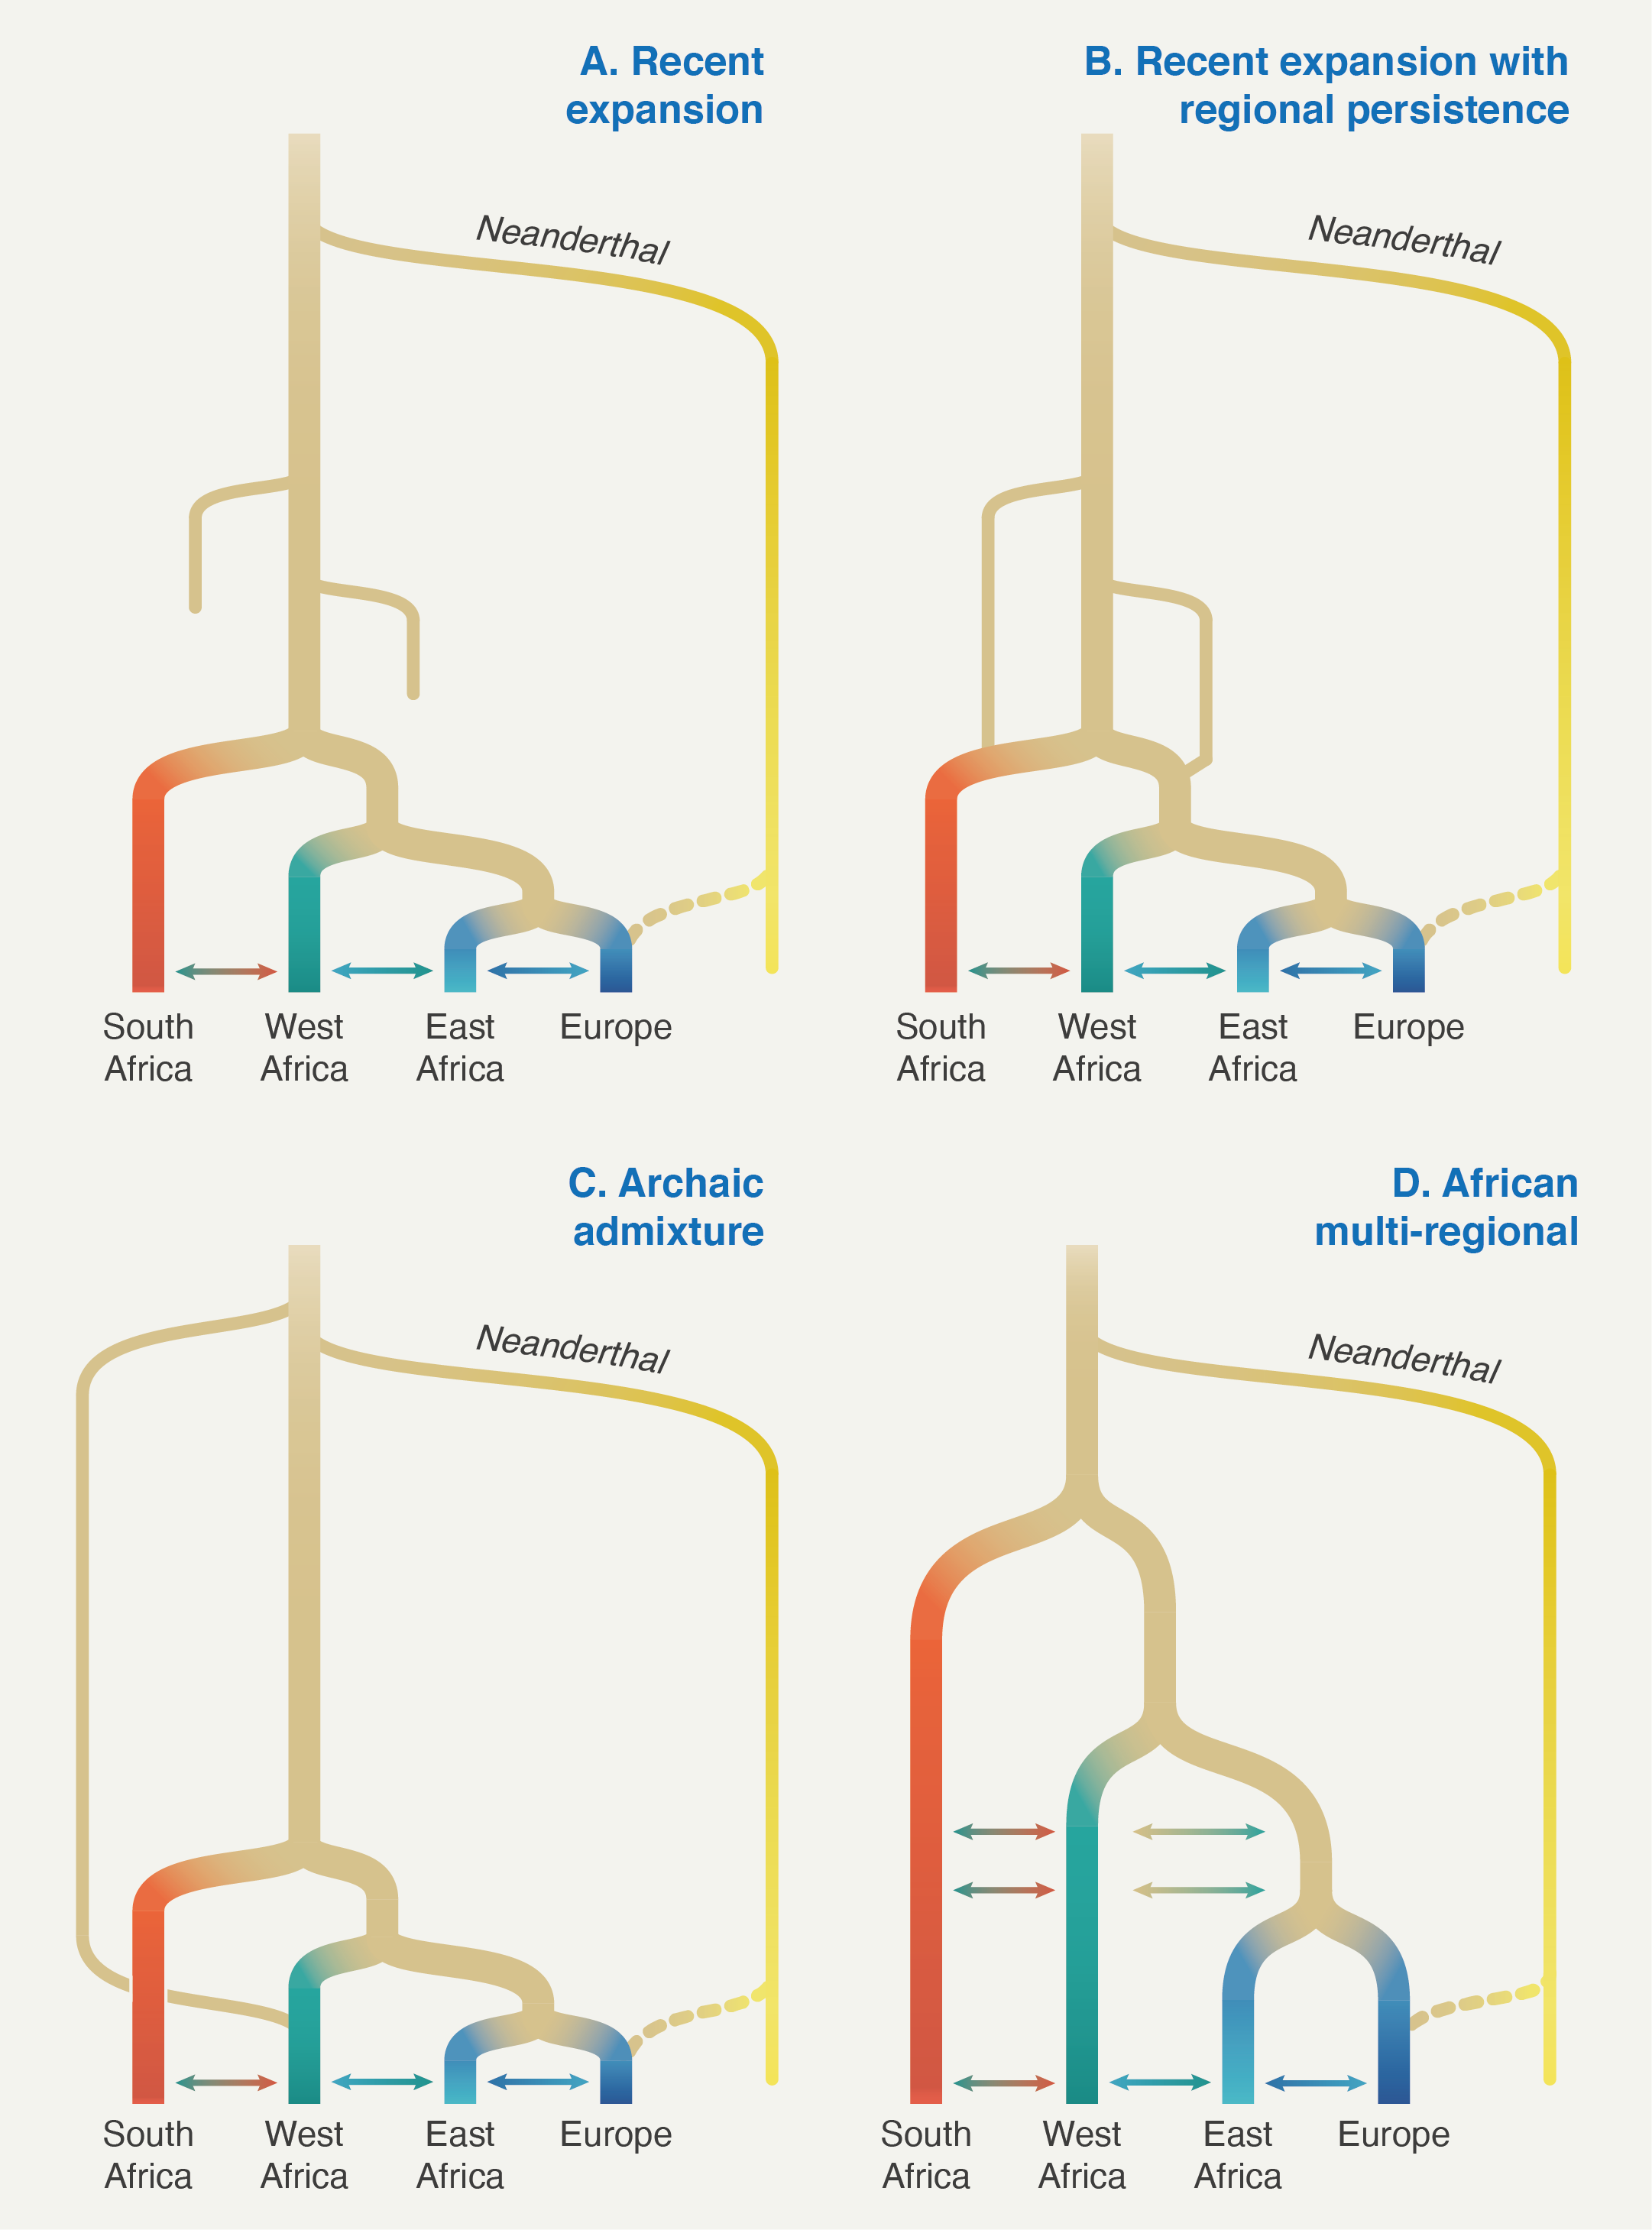
\includegraphics[width=0.65\textwidth]{figures/supp-possible-models.png}
    \caption{
        \textbf{Proposed models of early human history in Africa.}
    }
    \label{fig:supp-possible-models}
\end{figure}

\begin{figure}[ht]
    \centering
    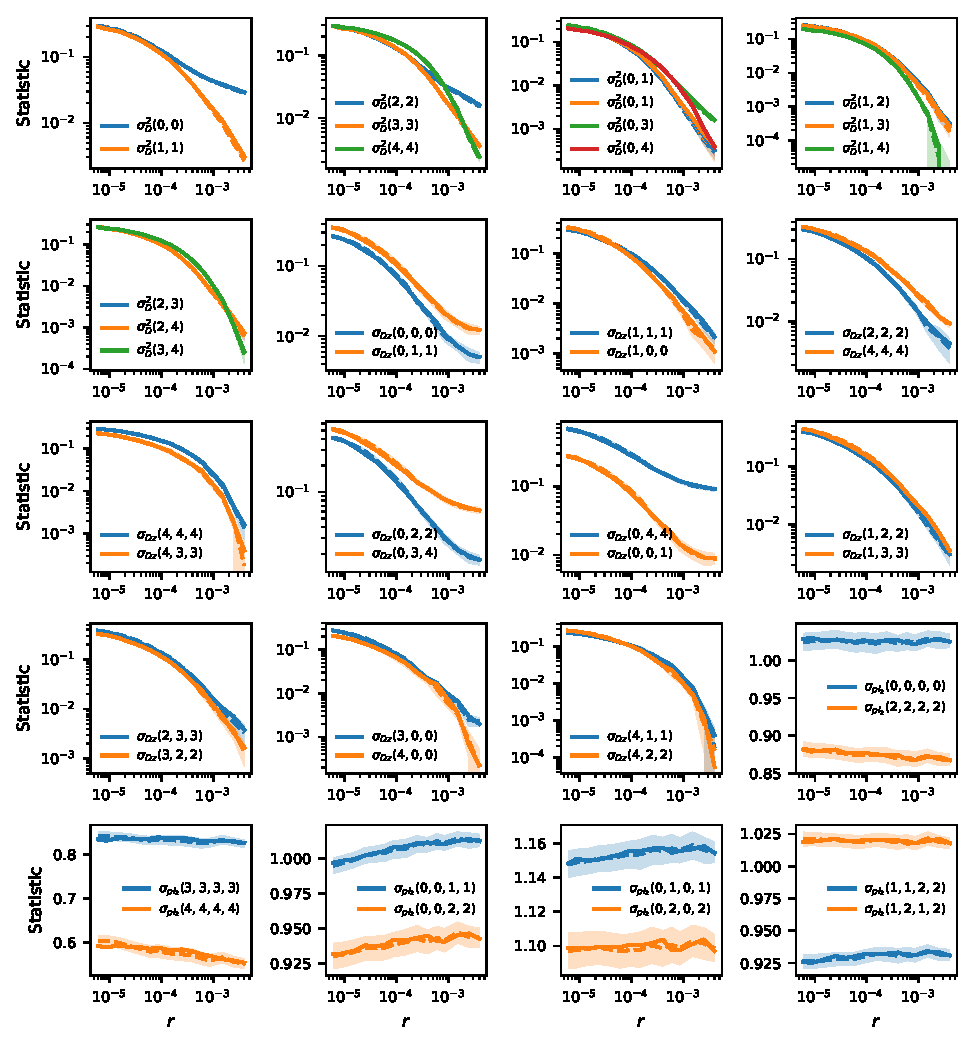
\includegraphics{figures/supp-omni-hapmap-comparison.pdf}
    \caption{
        \textbf{Comparison of LD statistics parsed using two recombination maps}
        The recombination map determines genetic distances between pairs of SNPs,
        so using different maps could result in systematic biases in parsed
        statistics if the maps differ significantly. Here, the solid lines are
        statistics parsed using the HapMapII recombination map, and dashed lines
        are using the OMNI-YRI map. Shading represents 95\% confidence intervals
        from the OMNI map. These two maps results in LD statistics that are
        indistinguishable from one another. Notations for each statistic are
        described in section~\ref{sec:supp-ld-stats} and indexed by populations
        (0: Nama, 1: Mende, 2: Gumuz, 3: Amhara/Oromo, 4: British).
    }
    \label{fig:supp-omni-hapmap-comparison}
\end{figure}

\begin{figure}[ht]
    \centering
    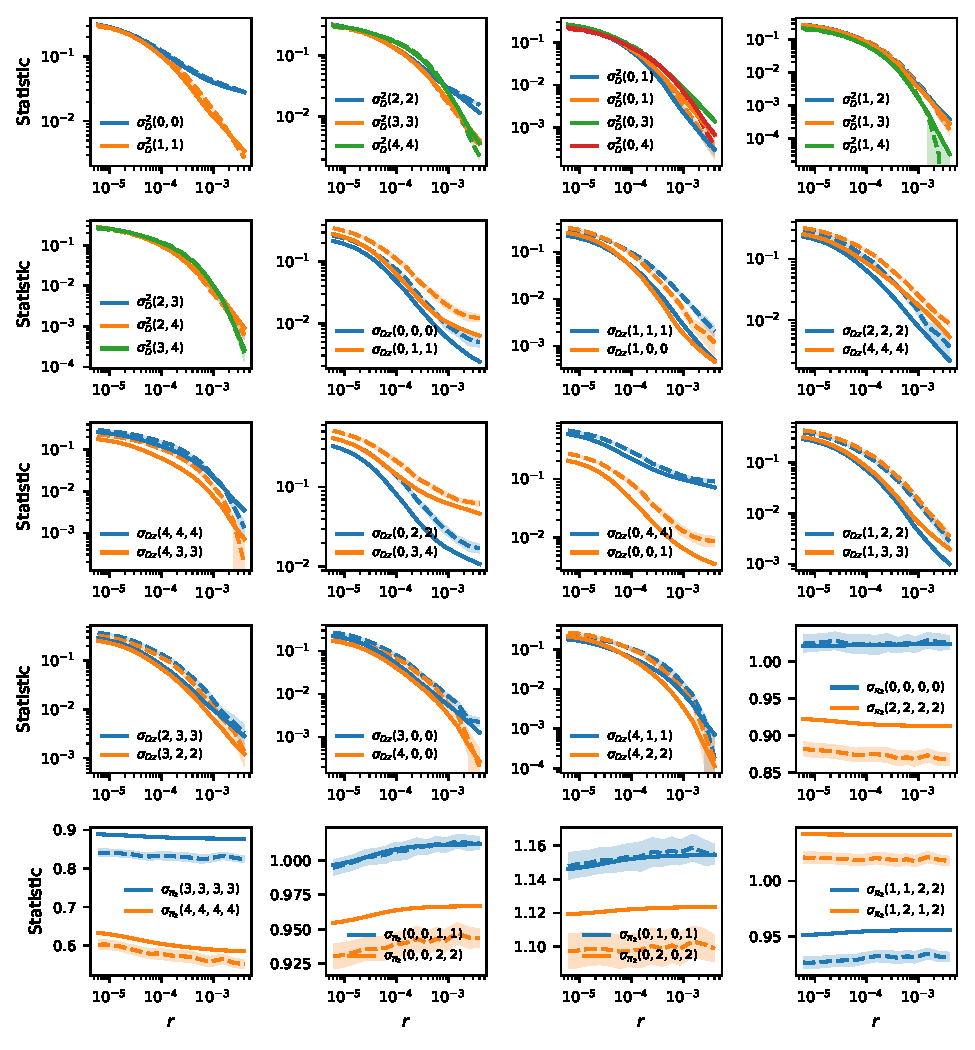
\includegraphics{figures/supp-single-origin-fits.pdf}
    \caption{
        \textbf{Single-origin model fit to LD statistics.}
        Predicted vs observed two-locus statistics as a function of genetic
        distance for the single-origin model. Each panel represents a different
        set of two-locus statistics. Solid lines represent estimates using the
        single-origin model. Dashed lines represent observed statistics.
        Notation and indexing of statistics are described in the
        Fig.~\ref{fig:supp-omni-hapmap-comparison} caption.
    }
    \label{fig:supp-single-origin-fits}
\end{figure}

\begin{figure}[ht]
    \centering
    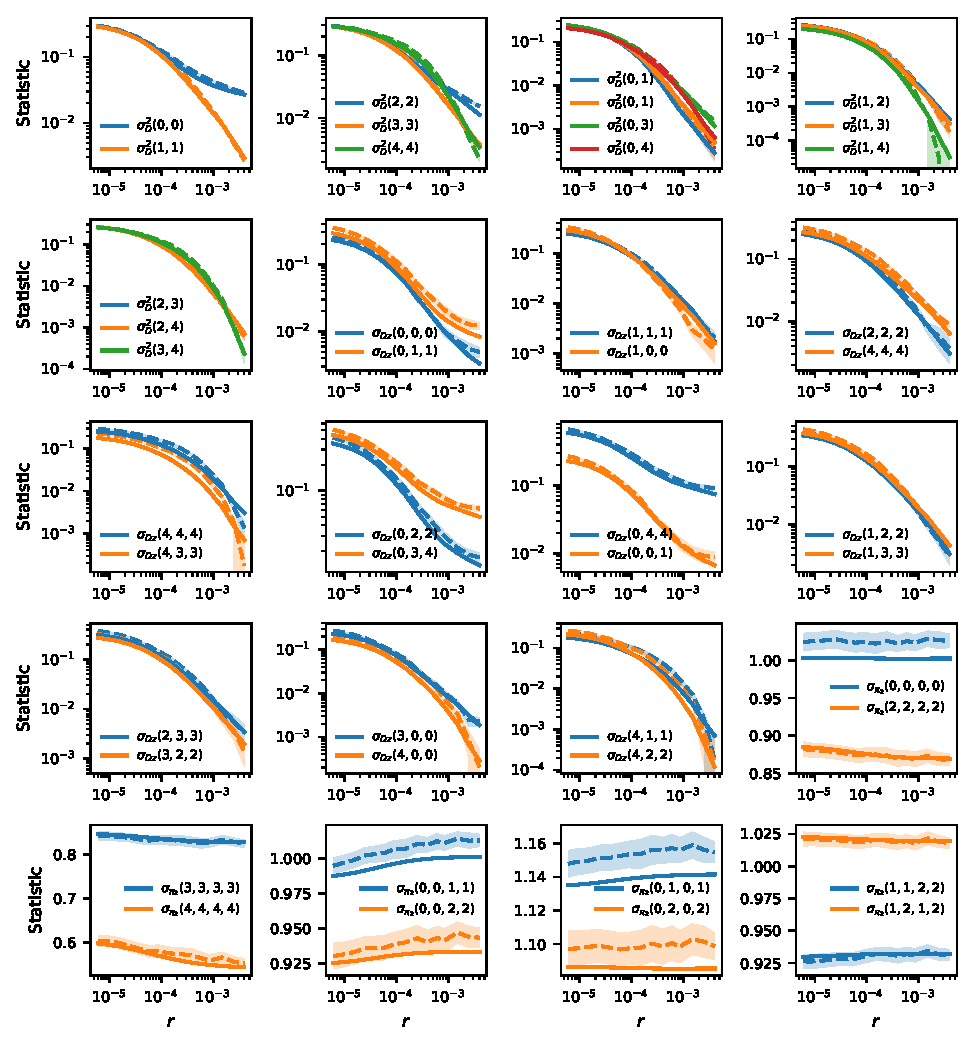
\includegraphics{figures/supp-continuous-migration-fits.pdf}
    \caption{
        \textbf{Continuous-migration model fit to LD statistics.}
        Predicted vs observed two-locus statistics as a function of genetic
        distance for the continuous-migration model. Each panel represents a different
        set of two-locus statistics. Solid lines represent estimates using the
        continuous-migration model. Dashed lines represent observed statistics.
        Notation and indexing of statistics are described in the
        Fig.~\ref{fig:supp-omni-hapmap-comparison} caption.
    }
    \label{fig:supp-continuous-migration-fits}
\end{figure}

\begin{figure}[ht]
    \centering
    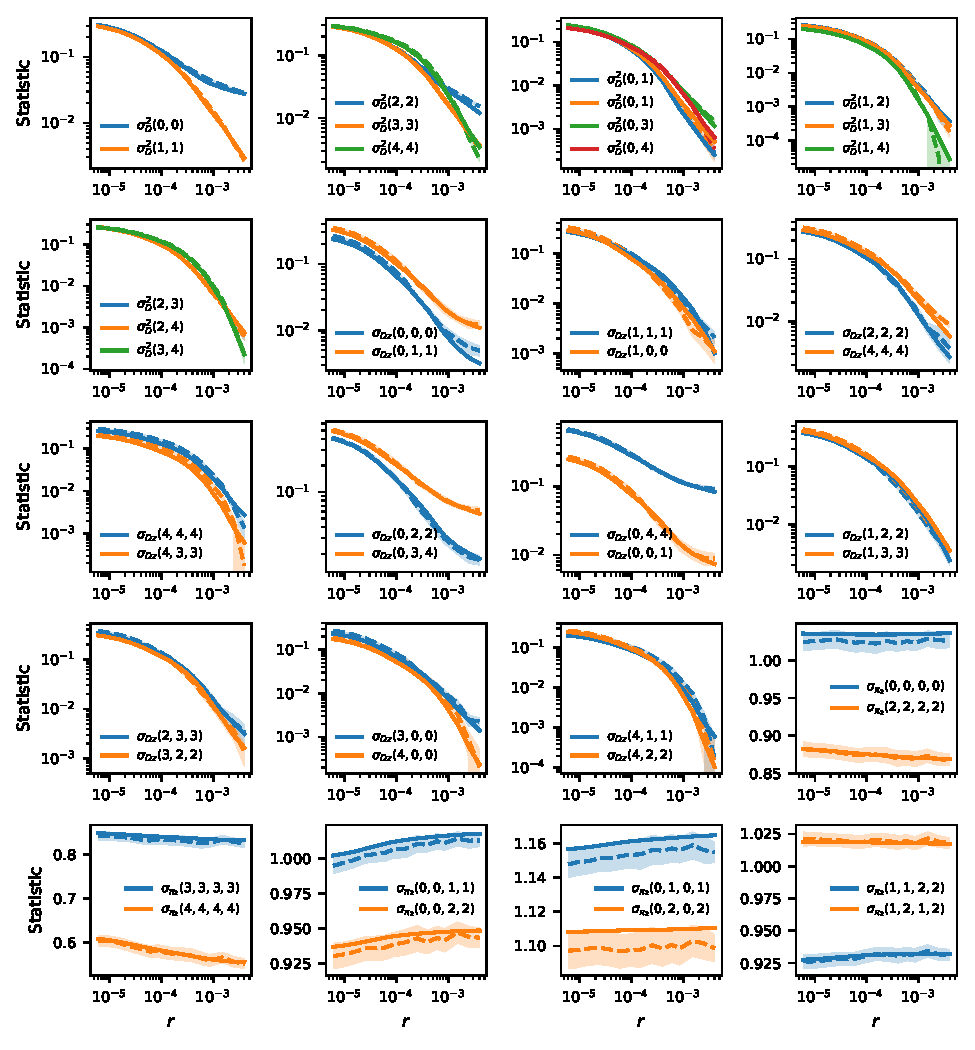
\includegraphics{figures/supp-merger-without-stem-migration-fits.pdf}
    \caption{
        \textbf{Merger-without-stem-migration model fit to LD statistics.}
        Predicted vs observed two-locus statistics as a function of genetic
        distance for the merger-without-stem-migration model. Each panel
        represents a different set of two-locus statistics.
        Solid lines represent estimates using the
        merger-without-stem-migration model.
        Dashed lines represent observed statistics.
        Notation and indexing of statistics are described in the
        Fig.~\ref{fig:supp-omni-hapmap-comparison} caption.
    }
    \label{fig:supp-merger-without-stem-migration-fits}
\end{figure}

\begin{figure}[ht]
    \centering
    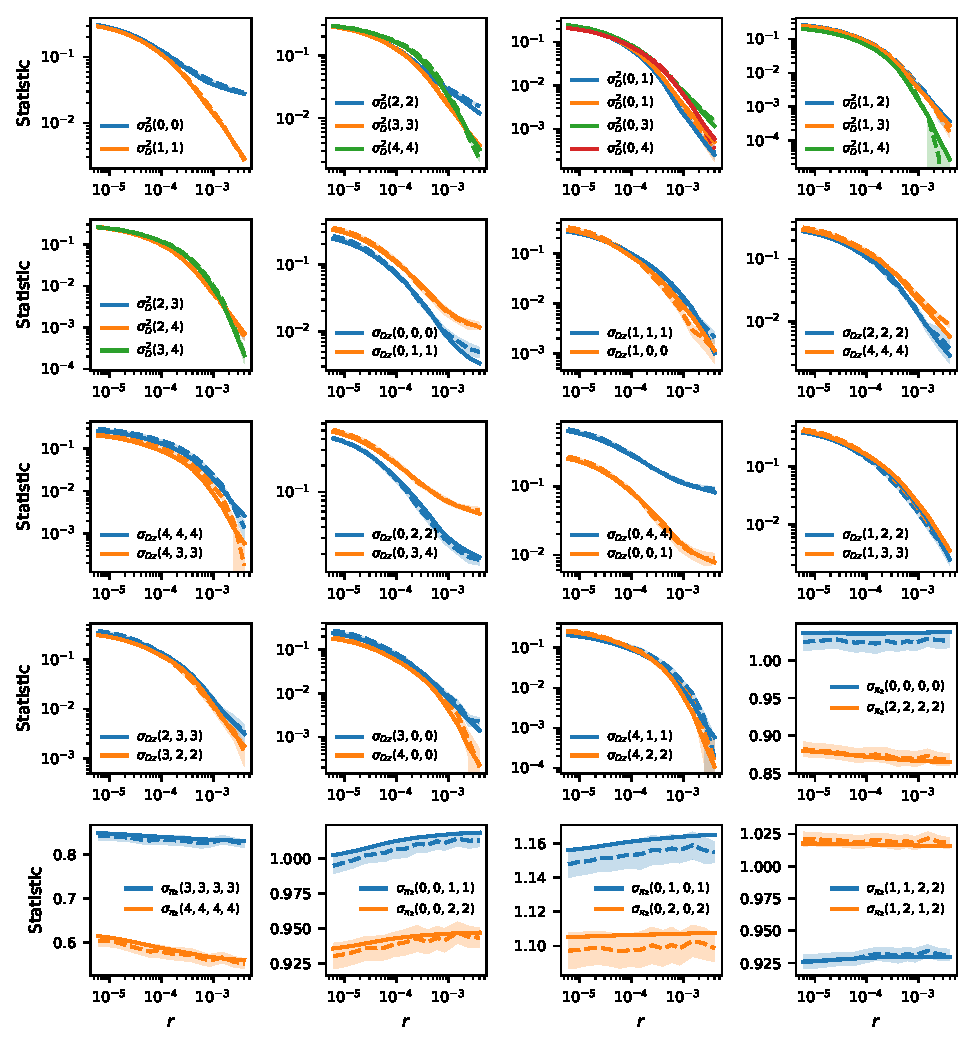
\includegraphics{figures/supp-merger-with-stem-migration-fits.pdf}
    \caption{
        \textbf{Merger-with-stem-migration model fit to LD statistics.}
        Predicted vs observed two-locus statistics as a function of genetic
        distance for the merger-with-stem-migration model. Each panel
        represents a different set of two-locus statistics.
        Solid lines represent estimates using the
        merger-with-stem-migration model.
        Dashed lines represent observed statistics.
        Notation and indexing of statistics are described in the
        Fig.~\ref{fig:supp-omni-hapmap-comparison} caption.
    }
    \label{fig:supp-merger-with-stem-migration-fits}
\end{figure}

\begin{figure}[ht]
    \centering
    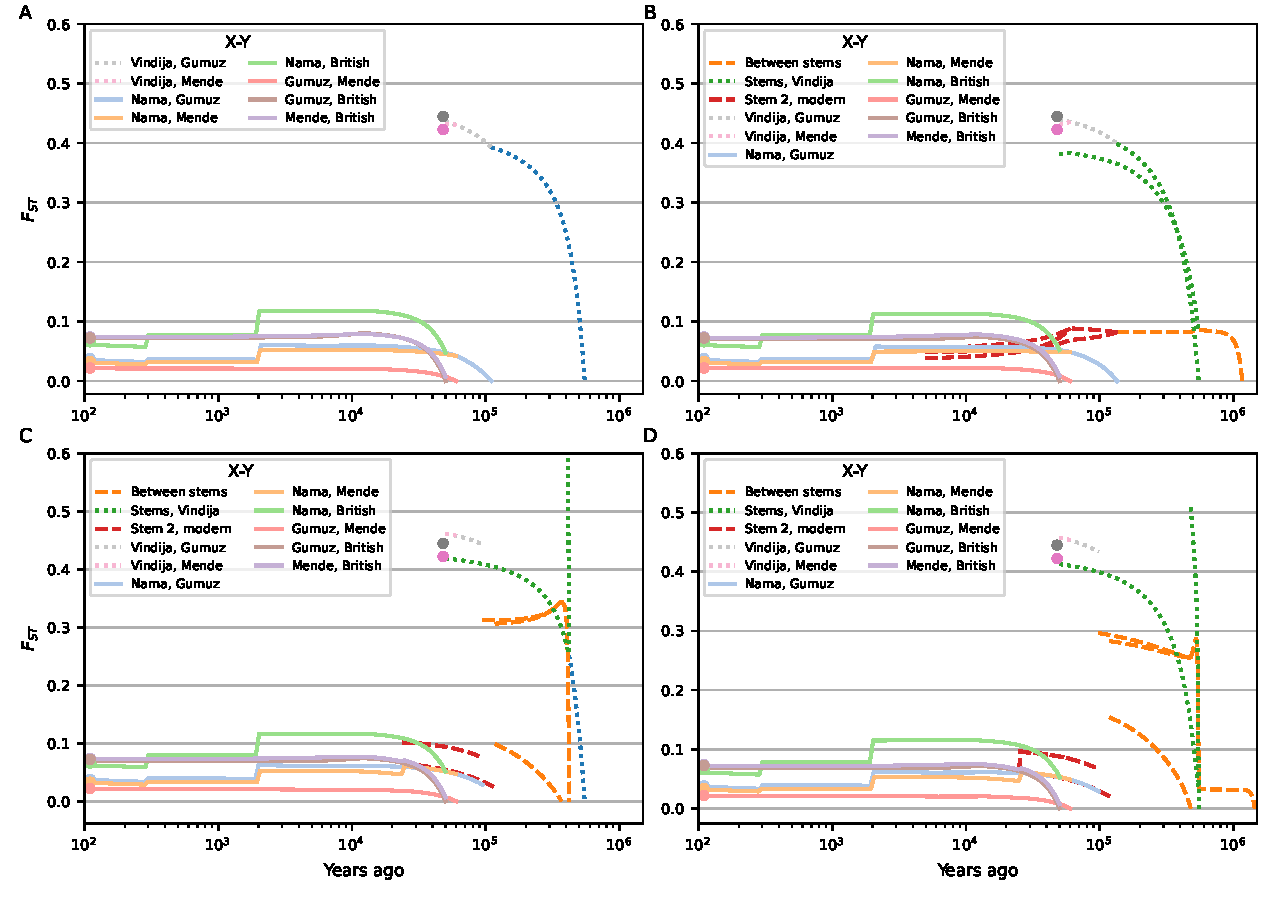
\includegraphics[width=\textwidth]{figures/supp-fsts-all-models.pdf}
    \caption{
        \textbf{Predicted \bm{$F_{ST}$} between contemporaneous populations over time.}
        All models (A: single origin, B: continuous migration, C: merger without stem
        migration, D: merger with stem migration) match observed $F_{ST}$ between
        sampled populations. The continuous-migration model predicts that human stem
        populations remain genetically similar, while the merger with and without
        stem migration models predict a period of increased $F_{ST}$ between ancestors
        of modern humans. This is largely due to the very small inferred $N_e$ in one of
        the stem branches, which leads to a rapid increase in differentiation due to
        drift.
    }
    \label{fig:supp-FST-panels}
\end{figure}

\begin{figure}[ht]
    \centering
    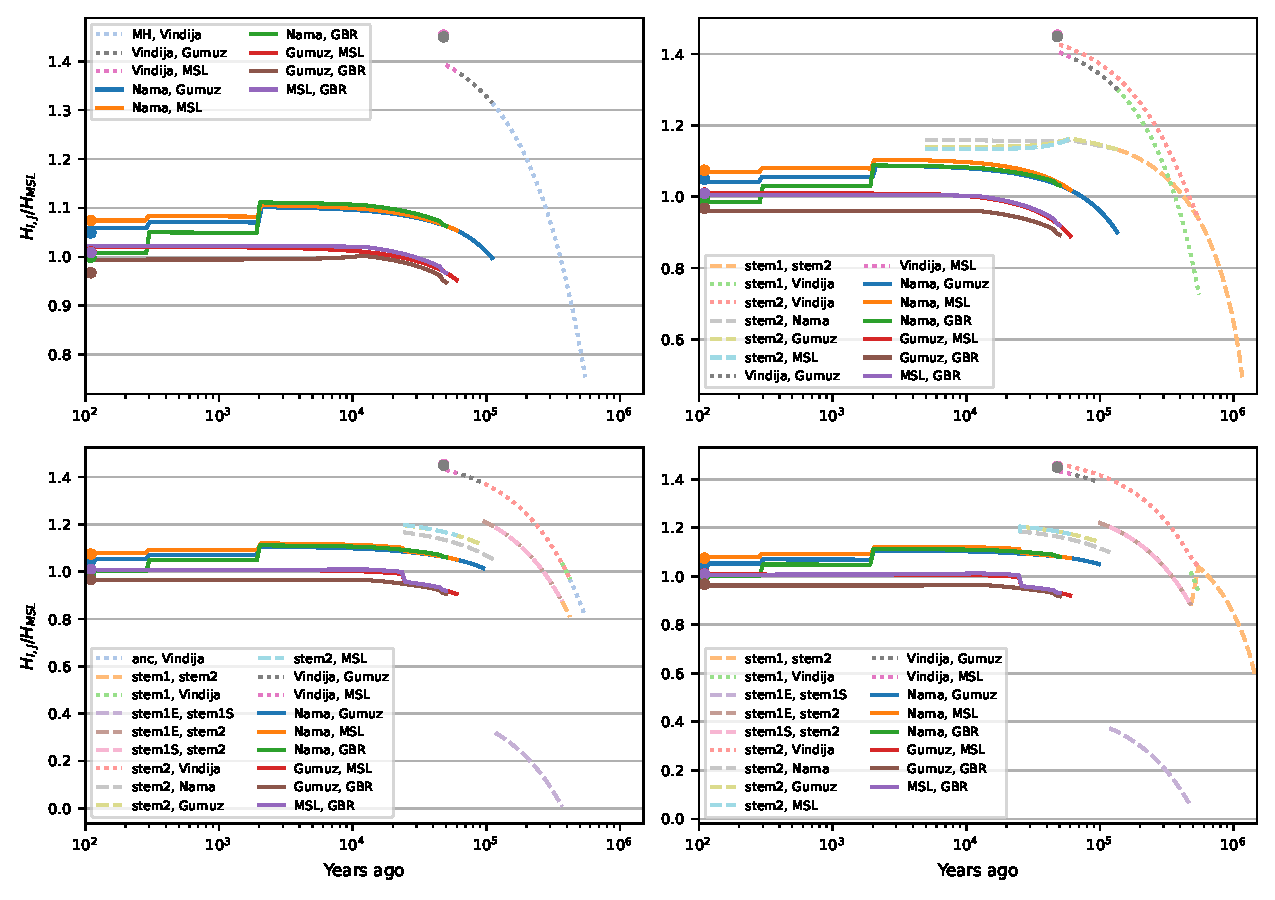
\includegraphics[width=\textwidth]{figures/supp-h12s-all-models.pdf}
    \caption{
        \textbf{Predicted pairwise differentiation between contemporaneous populations.}
        $H_{i,j}$ is the predicted pairwise differentiaion between two populations,
        which we normalize by the observed pairwise diversity in the Mende sample.
        The single-origin model (A) shows larger deviations between observed and
        expected differentiation than the models with early human structure
        (B: continuousmigration, C: merger without stem migration, D: merger with 
        stem migration). In the merger models (C and D), while $F_{ST}$ is large
        between early stems due to the sharp bottleneck in one of those branches,
        the pairwise differences are comparable to the continuous-migration model.
        Stem 1E and Stem 1S have low differentiation, as the bottleneck in Stem 1
        (which they both split from) sharply reduces diversity by the time of the
        split. This has the effect of large $F_{ST}$ but small $H_{i,j}$.
    }
    \label{fig:supp-h12-panels}
\end{figure}

\begin{figure}[ht]
    \centering
    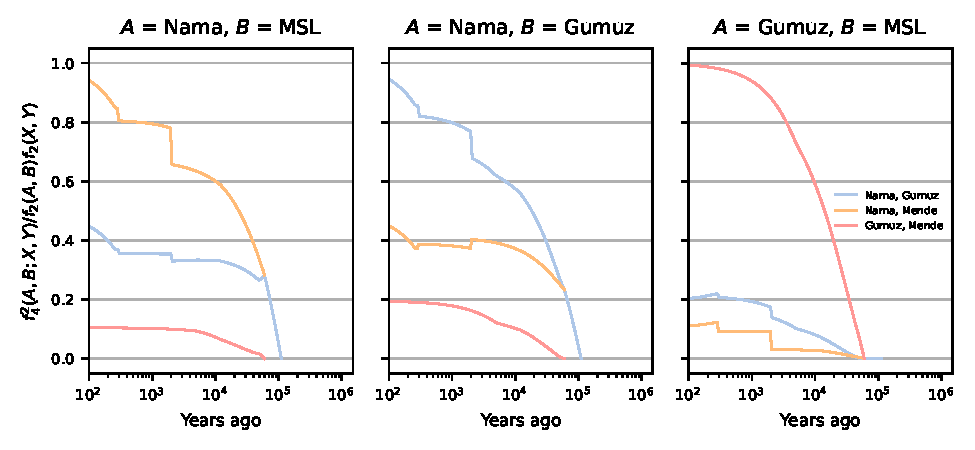
\includegraphics{figures/supp-f4s-single-origin.pdf}
    \caption{
        \textbf{Predicted \bm{$f_4$} between pairs of modern populations
        and ancient branches from the single-origin model.}
        $f_4(A, B; X, Y)/f_2(A, B)f_2(X, Y)$ is interpreted as the proportion of the
        amount of drift between sampled populations $A$ and $B$ that aligns with
        drift between populations $X$ and $Y$, sampled in the past
        (see Section~\ref{sec:f4}). In the single-origin model, nearly all
        differentiation between the Nama, Mende, and Gumuz populations arises
        after the divergence events, so normalized $f_4$ decays to zero by the
        time of those divergences.
    }
    \label{fig:supp-f4s-single-origin}
\end{figure}

\begin{figure}[ht]
    \centering
    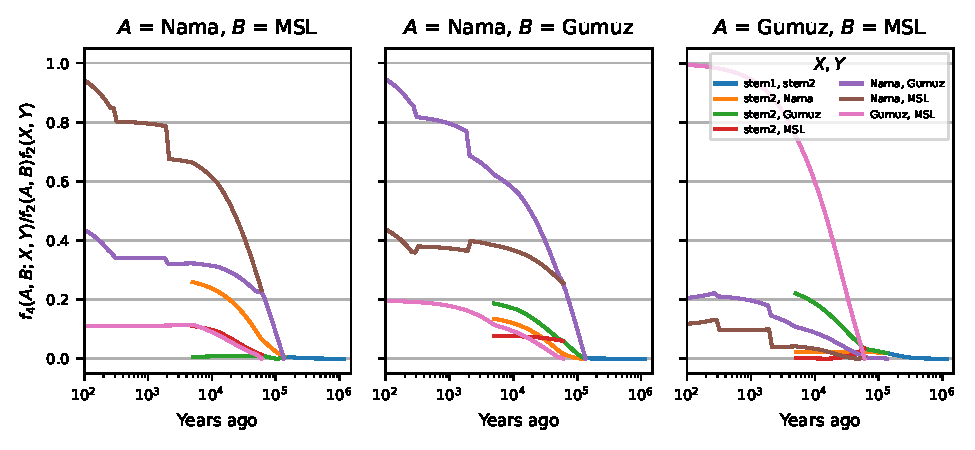
\includegraphics{figures/supp-f4s-continuous-migration.pdf}
    \caption{
        \textbf{Predicted \bm{$f_4$} between pairs of modern populations
        and ancient branches from the continuous-migration model.}
        Despite population structure inferred to have extended up to 1Ma
        into the past, differentiation between modern African populations
        only traces back to differentiation between ancestral populations
        $\sim$100-200ka, indicating that while stem populations were structured
        (Fig.~\ref{fig:supp-FST-panels}), differentiation due to that
        ancient structure does not contribute to differention between modern
        populations.
    }
    \label{fig:supp-f4s-continuous-migration}
\end{figure}

\begin{figure}[ht]
    \centering
    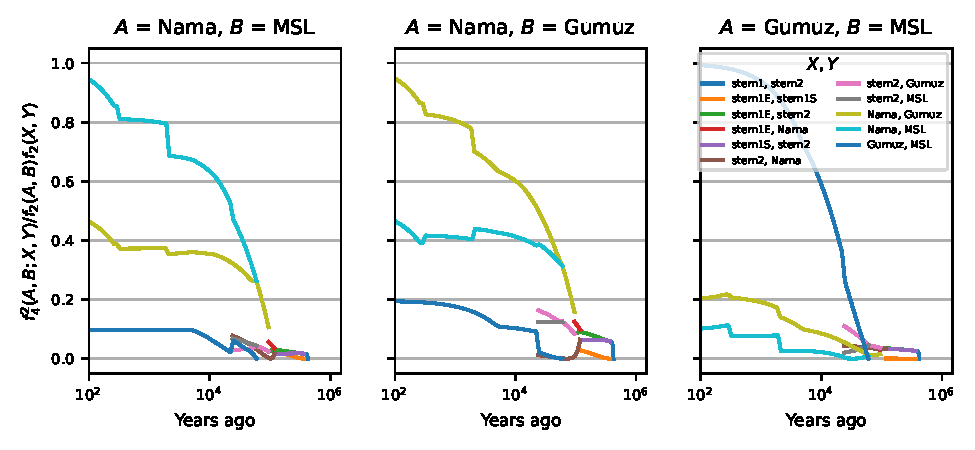
\includegraphics{figures/supp-f4s-merger-without-stem-migration.pdf}
    \caption{
        \textbf{Predicted \bm{$f_4$} between pairs of modern populations
        and ancient branches from the merger-without-stem-migration model.}
        Unlike the continuous-migration model, population structure in the stems
        following the divergence of Neanderthal and human ancestors results
        in differentiation among modern populations that aligns with drift
        between the stems. In this model, migration between stem populations
        is disallowed.
    }
    \label{fig:supp-f4s-merger-without-stem-migration}
\end{figure}

\begin{figure}[ht]
    \centering
    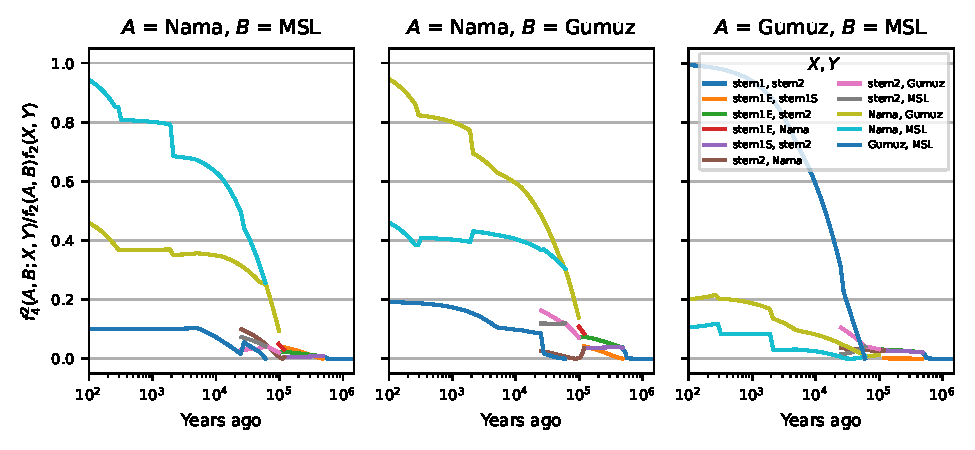
\includegraphics{figures/supp-f4s-merger-with-stem-migration.pdf}
    \caption{
        \textbf{Predicted \bm{$f_4$} between pairs of modern populations
        and ancient branches from the merger-with-stem-migration model.}
        Differentiation between modern present-day populations aligns with
        up to $\approx 5\%$ of the drift between stems, although some
        population pairs show even less shared drift.
    }
    \label{fig:supp-f4s-merger-with-stem-migration}
\end{figure}

\begin{figure}[ht]
    \centering
    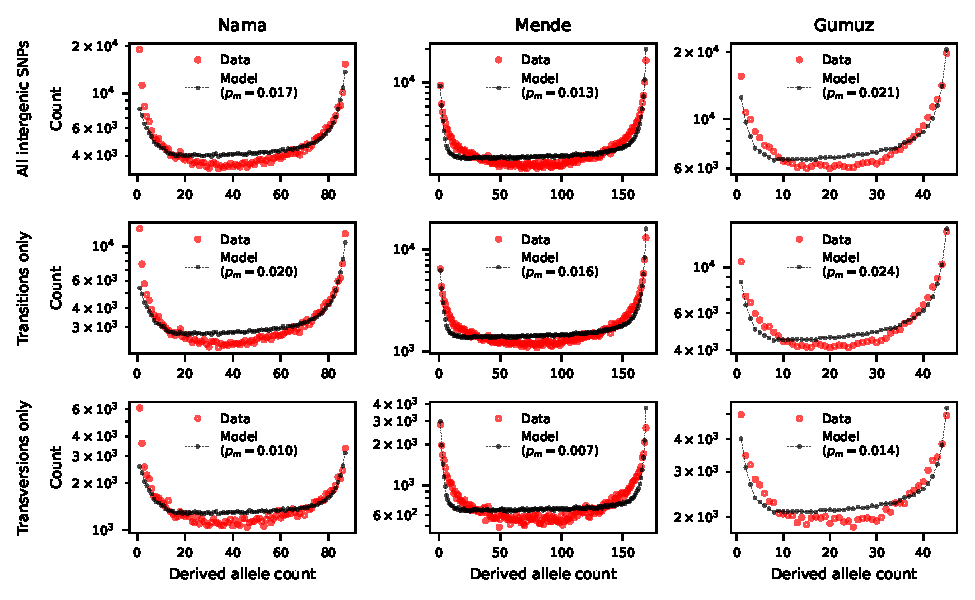
\includegraphics{figures/supp-csfs-single-origin.pdf}
    \caption{
        \textbf{Conditional SFS compared to single-origin model.}
        The single-origin model provides a poor fit to the observed cSFS in
        the Mende, Gumuz, and Nama. Ancestral state misidentification was
        inferred to be between 1 and $2\%$, and misidentification rates were
        consistent across model comparisons. Misidentification rates of
        transition-type mutations were roughly double that of transversion-type
        mutations, consistent with the higher mutation rates of transition
        mutations vs. transversions.
    }
    \label{fig:supp-csfs-single-origin}
\end{figure}

\begin{figure}[ht]
    \centering
    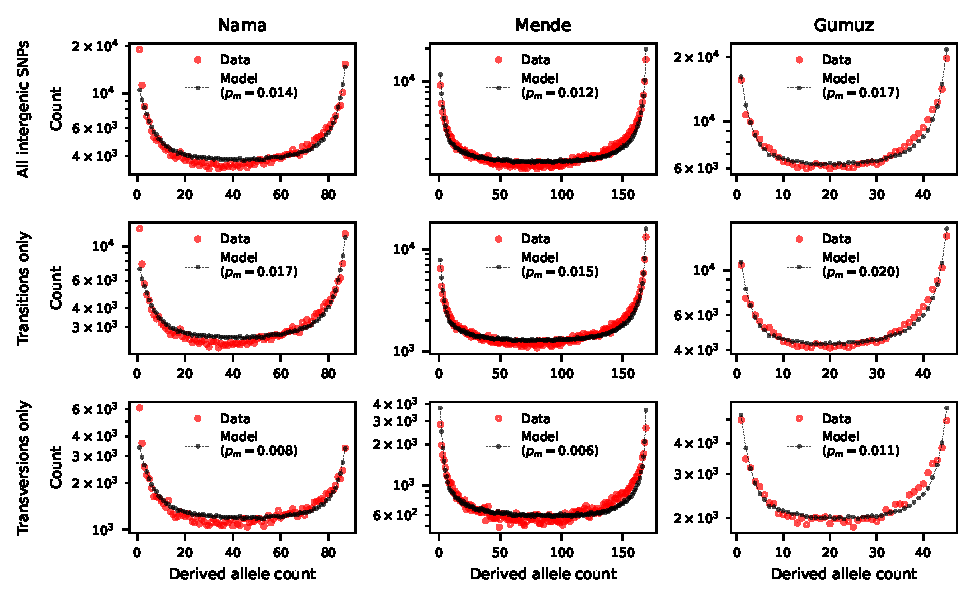
\includegraphics{figures/supp-csfs-continuous-migration.pdf}
    \caption{
        \textbf{Conditional SFS compared to continuous-migration model.}
        The continuous-migration model provides a better fit to the data than
        either the single-origin model or the merger-without-stem-migration
        model, although systematic deviations are still noticeable in each
        population.
    }
    \label{fig:supp-csfs-continuous-migration}
\end{figure}

\begin{figure}[ht]
    \centering
    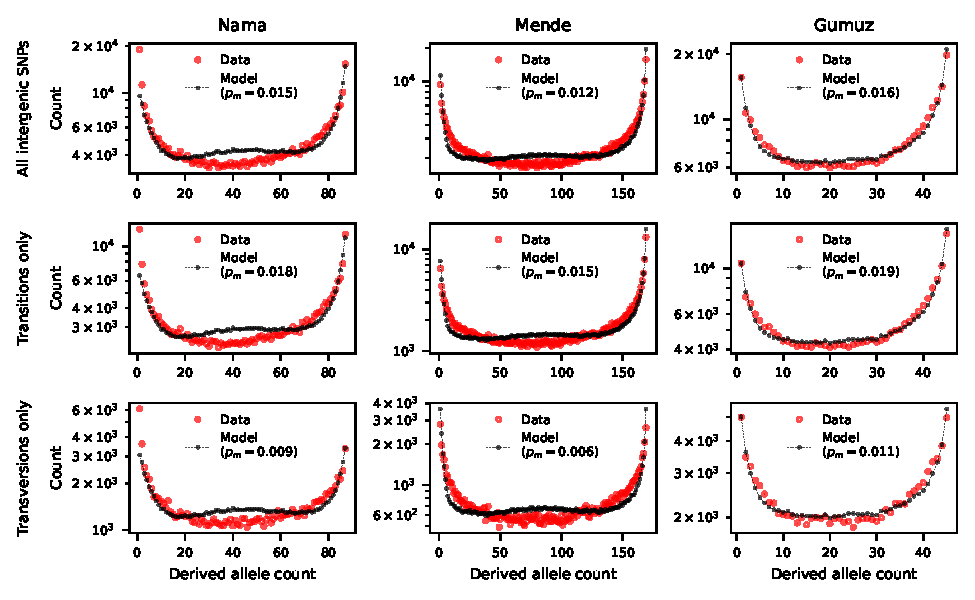
\includegraphics{figures/supp-csfs-merger-without-stem-migration.pdf}
    \caption{
        \textbf{Conditional SFS compared to merger-without-stem-migration model.}
        The excess of intermediate-frequency variants in the Nama and Mende
        cSFS results in a poorer fit to the cSFS compared to the continuous-migration
        and merger-with-stem-migratino models. Along with the poorer likelihood this
        model provides to the two-locus statistics, validation usin the cSFS
        disfavors a model with strict isolation between stem populations.
    }
    \label{fig:supp-csfs-merger-without-stem-migration}
\end{figure}

\begin{figure}[ht]
    \centering
    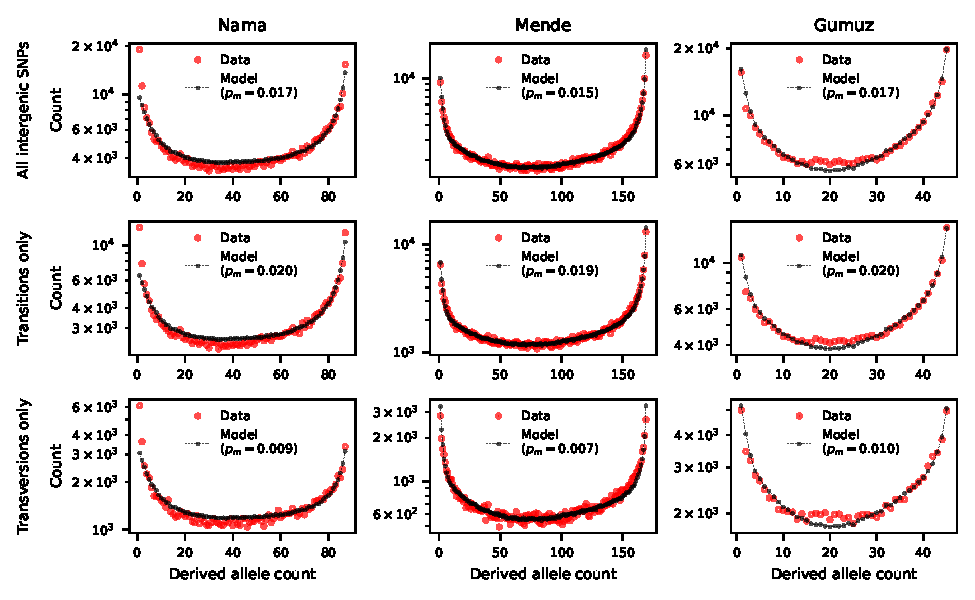
\includegraphics{figures/supp-csfs-merger-with-stem-migration.pdf}
    \caption{
        \textbf{Conditional SFS compared to merger-with-stem-migration model.}
        The merger-with-stem-migration model, in addition to providing the best
        fit to heterozygosity and LD statistics, provided the best fit to the cSFS
        in the Nama, Gumuz, and Mende populations. Rates of ancestral state
        misidentification were consistent across each comparison, with the
        ancestral state of transversion mutations estimated to be $0.7-1.0\%$, and
        that of transition mutations estimated to be $1.9-2.0\%$. These
        misidentification rates are consistent with the known difference in mutation
        rates between transitions and transversions, as well as other SFS-based
        inferences in humans using the Thousand Genomes data and the 6-primate
        alignment (see Methods).
    }
    \label{fig:supp-csfs-merger-with-stem-migration}
\end{figure}

\begin{figure}[ht]
    \centering
    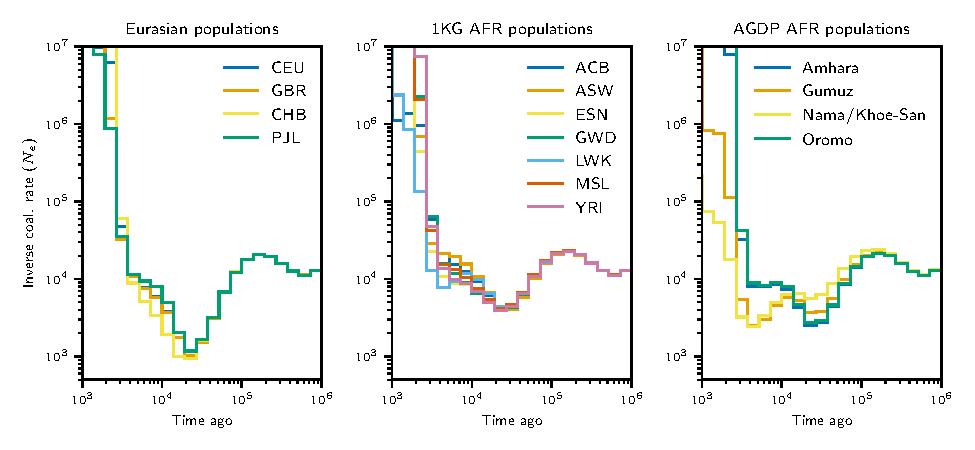
\includegraphics{figures/supp-relate-iicr-data}
    \caption{
        \textbf{Inverse instantaneous coalescence rates inferred from the data.}
        Using combined data from the Thousand Genomes Project and the AGRP,
        we reconstructed gene genealogies using Relate and calculated the
        inverse instantaneous coalescence rate for samples within each population.
        (A) Eurasian populations (CEU: European American, GBR: British,
        CHB: Han Chinese, PJL: Punjabi), (B) Thousand Genomes African populations
        (ACB: Afro-Caribbean, ASW: African American, ESN: Esan, GWD: Gambian,
        LWK: Luhya, MSL: Mende, YRI: Yoruba), (C) AGRP populations.
    }
    \label{fig:supp-iicr-data}
\end{figure}

\begin{figure}[ht]
    \centering
    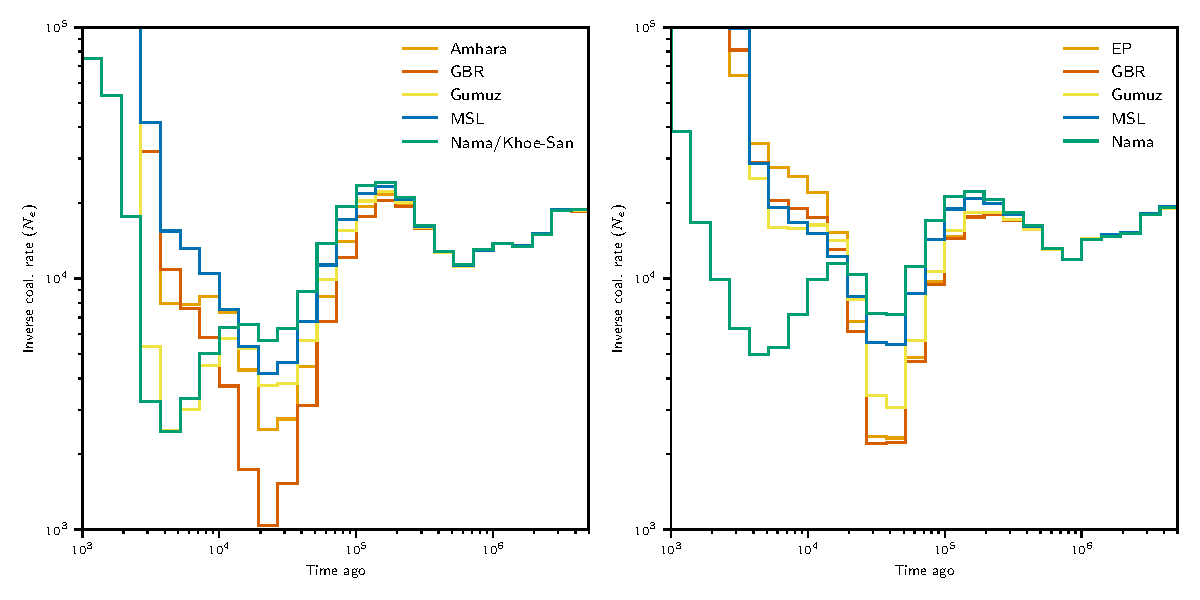
\includegraphics[width=\textwidth]{figures/supp-relate-iicr-data-full-and-subset}
    \caption{
        \textbf{Inverse instantaneous coalescence rates inferred from the data,
        subset to focal populations in the model inferences.}
        Fig.~\ref{fig:supp-iicr-data} shows IICR curves from reconstructed
        genealogies inferred using a larger dataset (including nearly 1,200
        individuals) than the subset of populations we primarily focused on
        here. To assess the robustness of Relate-inferred genealogies and for a
        direct comparison to our inferred demographic models, we ran Relate on
        the 290 genomes from the Nama, Gumuz, Mende, Amhara/Oromo, and British.
        While the reconstructed IICR curves are qualitatively similar to those
        from the full dataset for these populations in the distant past, there
        are noticeable discrepancies over the recent history in the last 10s of
        thousands of years. Left: Relate run on full dataset, showing focal
        populations. Right: Relate run directly on the subset dataset of focal
        populations.
    }
    \label{fig:supp-iicr-data-subset}
\end{figure}

\begin{figure}[ht]
    \centering
    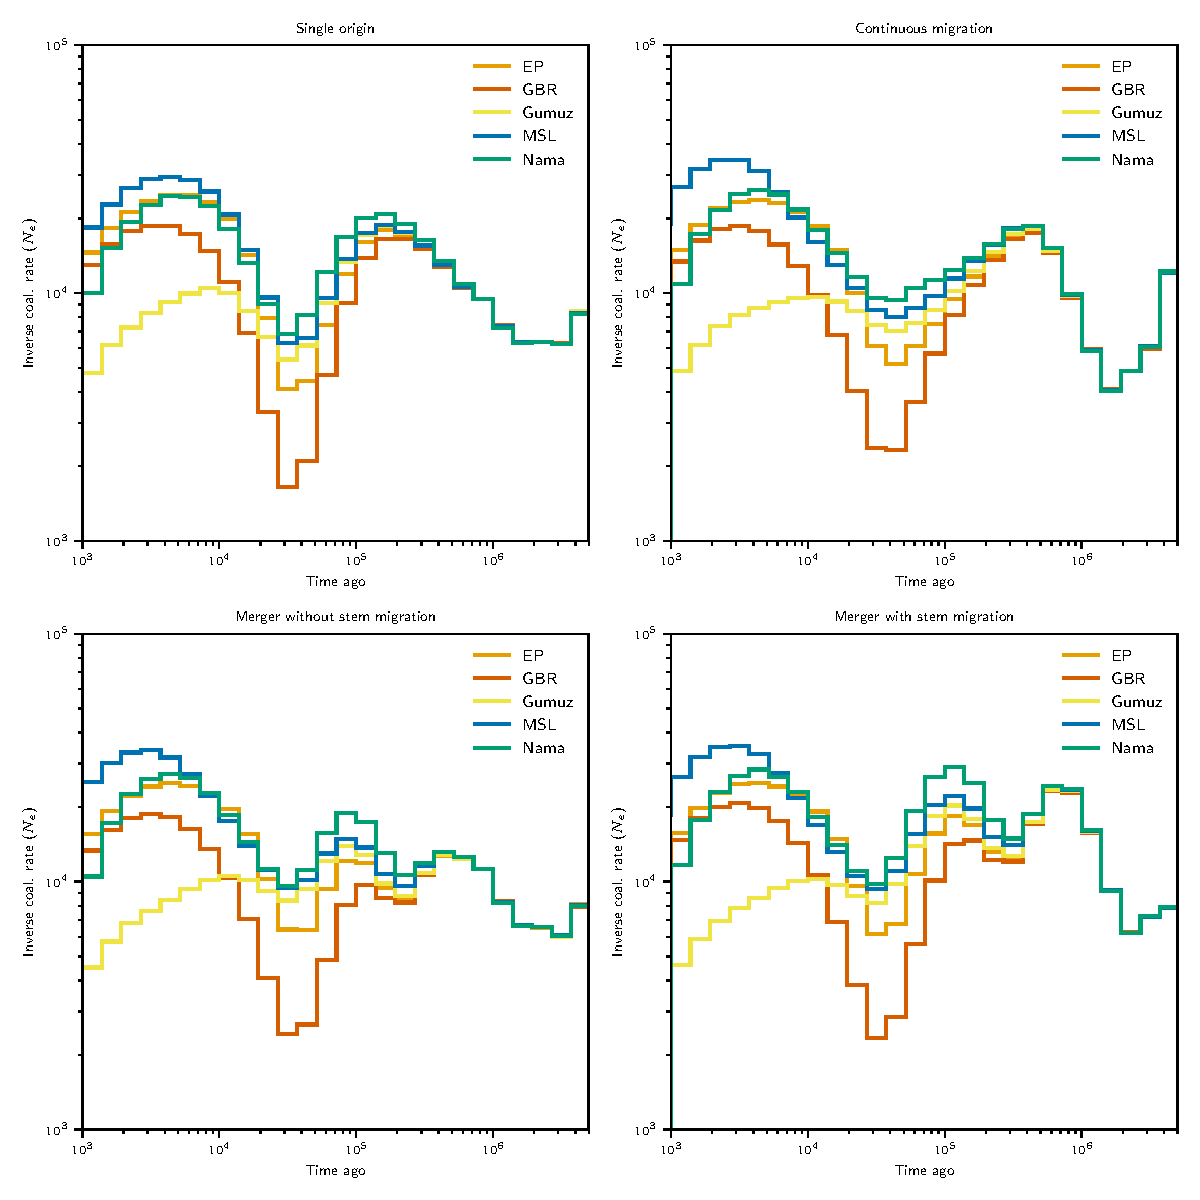
\includegraphics[width=\textwidth]{figures/supp-relate-iicr-simulation}
    \caption{
        \textbf{Inverse instantaneous coalescence rates reinferred from
        simulated data.} We simulated data under our four highlighted models,
        sampling the same number of individuals per population as the original
        dataset, and then ran Relate on each simulated dataset to reconstruct
        IICR curves for each. Each model has qualitatively different histories,
        particularly for the distant past with varying numbers and timings of
        oscillations. However, due to the discrepancies in reconstructed
        genealogies using even the same data as input
        (Figs.~\ref{fig:supp-iicr-data-subset} and \ref{fig:supp-rccr-data}),
        it is difficult to draw firm conclusions from qualitative comparisons
        between reconstructed genealogies.
    }
    \label{fig:supp-iicr-sim}
\end{figure}

\begin{figure}[ht]
    \centering
    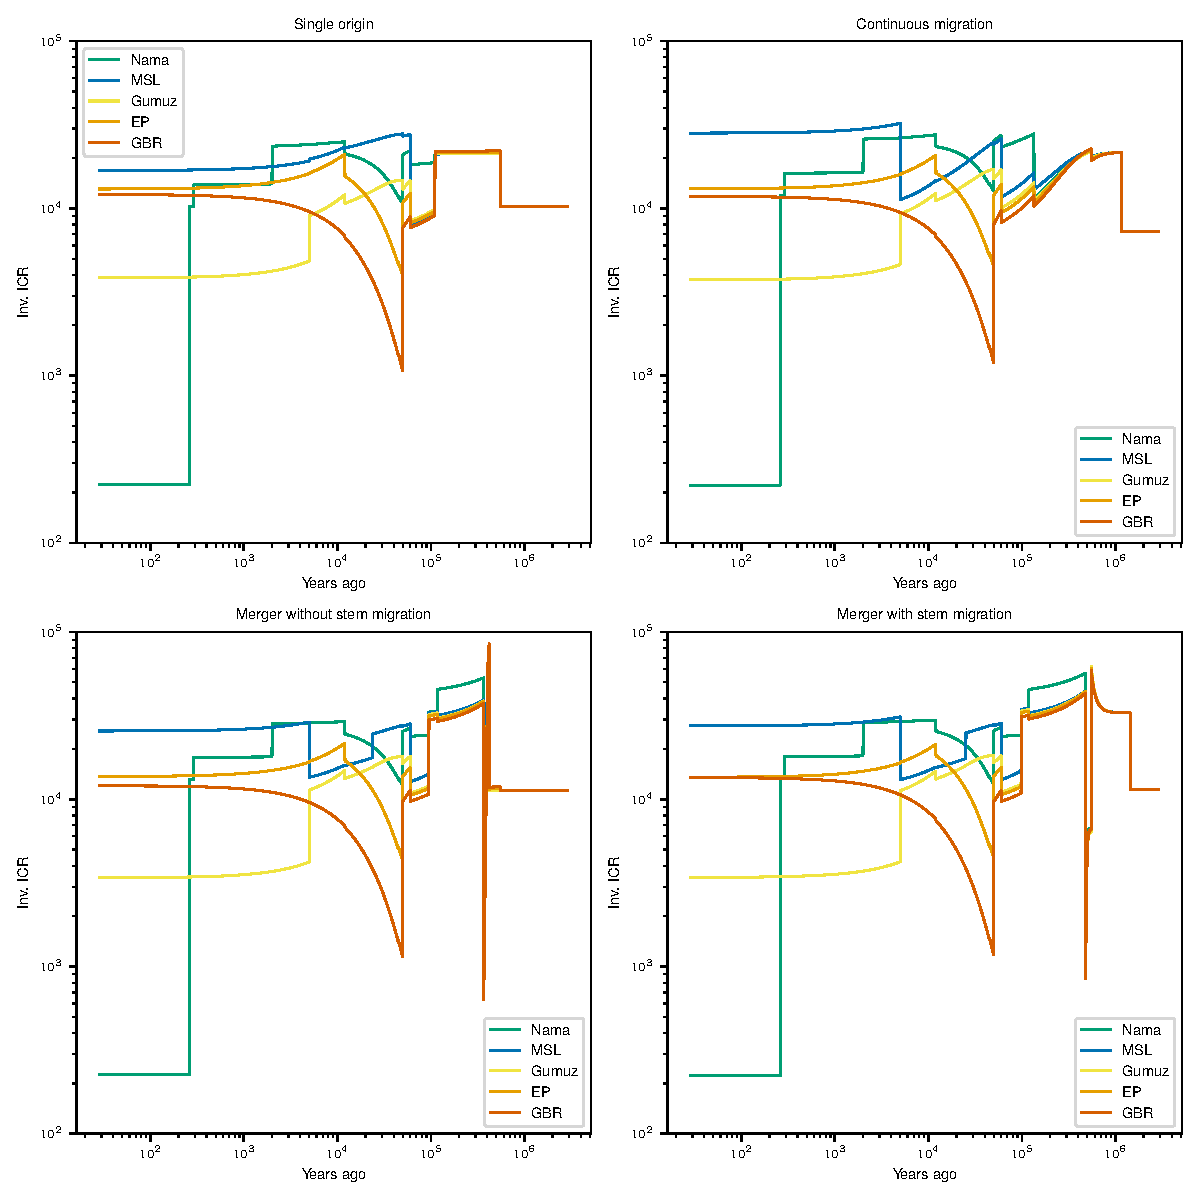
\includegraphics[width=\textwidth]{figures/supp-exp-coal-rates}
    \caption{
        \textbf{Expected inverse instantaneous coalescence rates from models.}
        The inferred demographic models specify population sizes, split times,
        and migration rates and events, making it possible to compute the exact
        expected IICR curve for each population. Due to discrete events
        (instantaneous size changes, for example), the models can produce
        non-smooth IICR curves, although each predicts a period of increased
        ``effective size'' in the past $\sim200-500$ka.
    }
    \label{fig:supp-iicr-exp}
\end{figure}

\begin{figure}[ht]
    \centering
    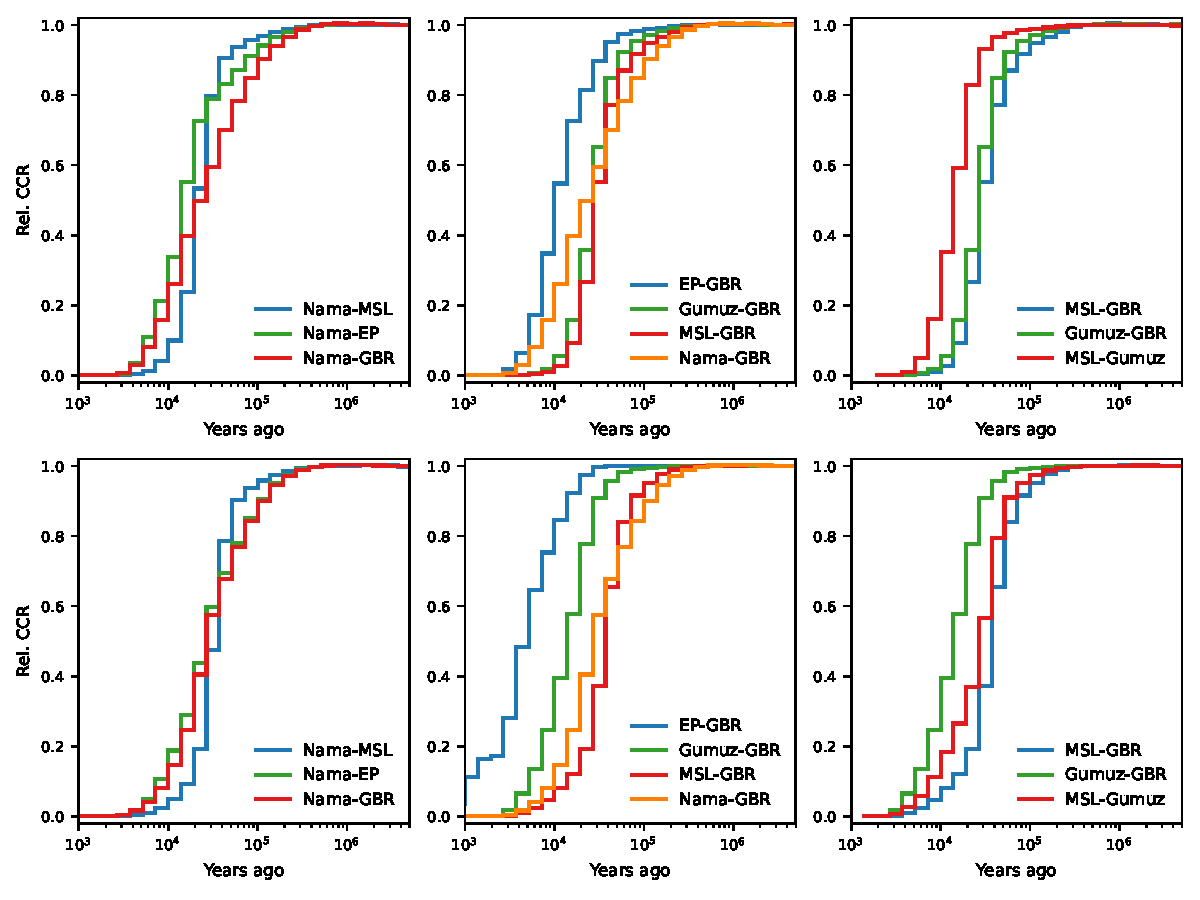
\includegraphics[width=\textwidth]{figures/supp-relate-rccr-data-full-and-subset}
    \caption{
        \textbf{Relative cross-coalescence rates inferred from the data.} Using
        the same reconstructed genealogies from Relate, we computed RCCR curves
        for pairs of populations using genealogies from the full dataset
        ($\sim1,200$ individuals) and the subset of focal populations (290
        individuals). Despite the overlap in samples, the two sets of inferred
        genealogies provided inconsistent RCCR, with both the timing and
        ordering of increased RCCR varying between the two datasets.
        Genealogies reconstructed from the full dataset provide a better match
        to each of inferred demographic models
        (Figs.~\ref{fig:supp-rccr-single-origin}--\ref{fig:supp-rccr-merger-with-stem-migration}).
    }
    \label{fig:supp-rccr-data}
\end{figure}

\begin{figure}[ht]
    \centering
    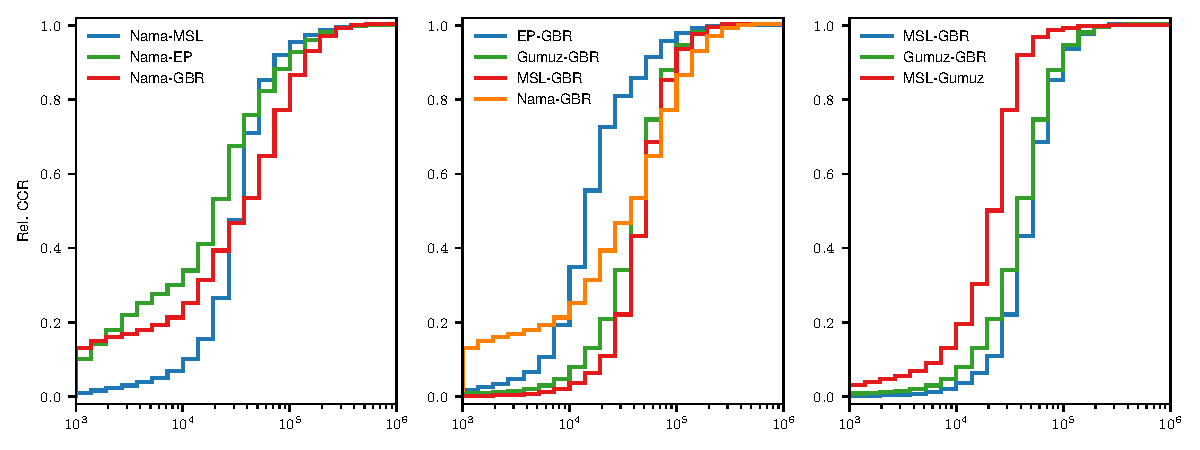
\includegraphics[width=\textwidth]{figures/supp-relate-rccr-single-origin}
    \caption{
        \textbf{Relative cross-coalescence rates reinferred from simulated data
        under the single-origin model.} RCCR curves from genealogies
        reconstructed from simulated data using Relate match those inferred
        from the full dataset (\label{fig:supp-rccr-data}, left) for distant
        timepoints. There are large discrepancies in the very recent history,
        where Relate and other genome-wide coalescence-based methods are known
        to be underpowered.
    }
    \label{fig:supp-rccr-single-origin}
\end{figure}

\begin{figure}[ht]
    \centering
    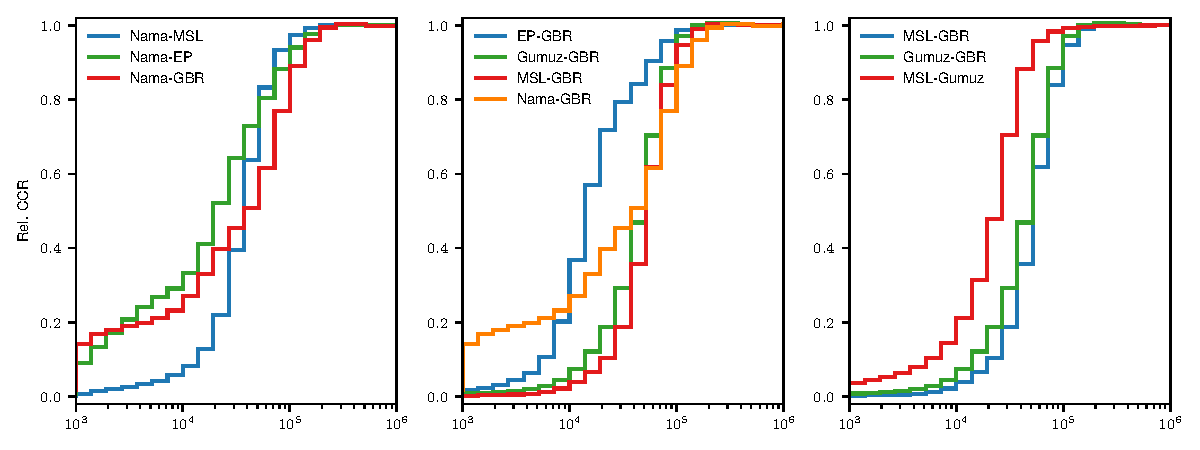
\includegraphics[width=\textwidth]{figures/supp-relate-rccr-continuous-migration}
    \caption{
        \textbf{Relative cross-coalescence rates reinferred from simulated data
        under the continuous-migration model.} RCCR curves from genealogies
        reconstructed from simulated data using Relate match those inferred
        from the full dataset (\label{fig:supp-rccr-data}, left) for distant
        timepoints. There are large discrepancies in the very recent history,
        where Relate and other genome-wide coalescence-based methods are known
        to be underpowered.
    }
    \label{fig:supp-rccr-continuous-migration}
\end{figure}

\begin{figure}[ht]
    \centering
    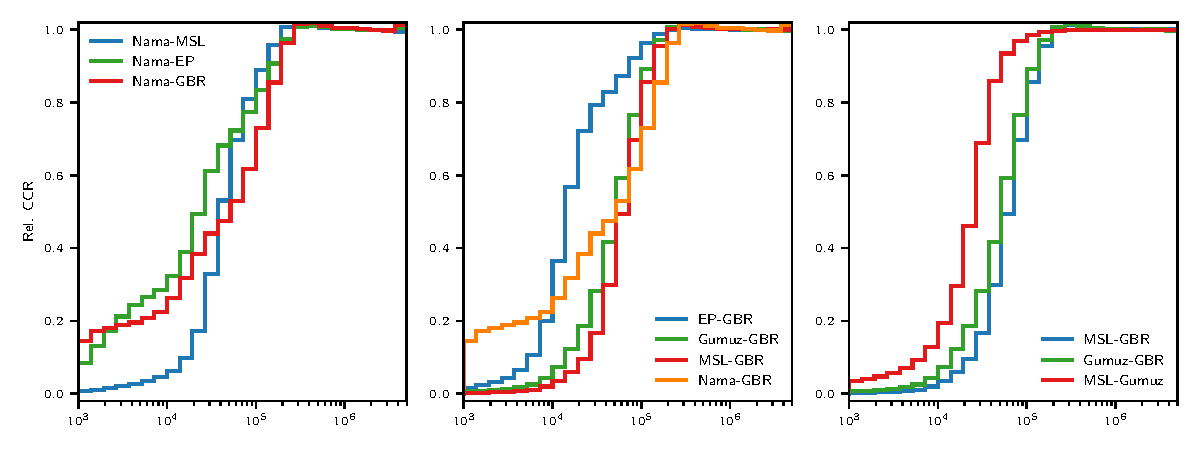
\includegraphics[width=\textwidth]{figures/supp-relate-rccr-merger-without-stem-migration}
    \caption{
        \textbf{Relative cross-coalescence rates reinferred from simulated data
        under the merger-without-stem-migration-model.} RCCR curves from genealogies
        reconstructed from simulated data using Relate match those inferred
        from the full dataset (\label{fig:supp-rccr-data}, left) for distant
        timepoints. There are large discrepancies in the very recent history,
        where Relate and other genome-wide coalescence-based methods are known
        to be underpowered.
    }
    \label{fig:supp-rccr-merger-without-stem-migration}
\end{figure}

\begin{figure}[ht]
    \centering
    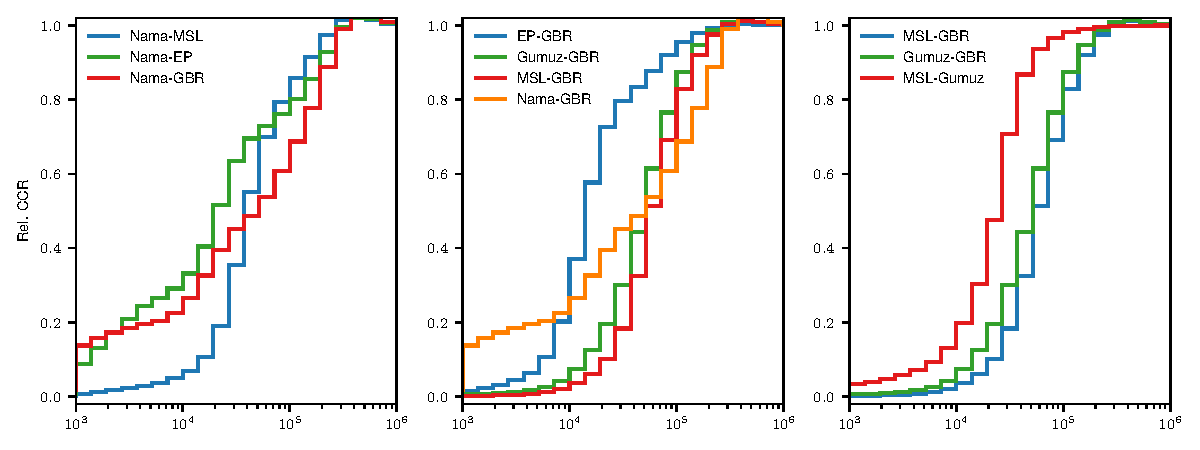
\includegraphics[width=\textwidth]{figures/supp-relate-rccr-merger-with-stem-migration}
    \caption{
        \textbf{Relative cross-coalescence rates reinferred from simulated data
        under the merger-with-stem-migration model.} RCCR curves from genealogies
        reconstructed from simulated data using Relate match those inferred
        from the full dataset (\label{fig:supp-rccr-data}, left) for distant
        timepoints. There are large discrepancies in the very recent history,
        where Relate and other genome-wide coalescence-based methods are known
        to be underpowered.
    }
    \label{fig:supp-rccr-merger-with-stem-migration}
\end{figure}

\begin{figure}[ht]
    \centering
    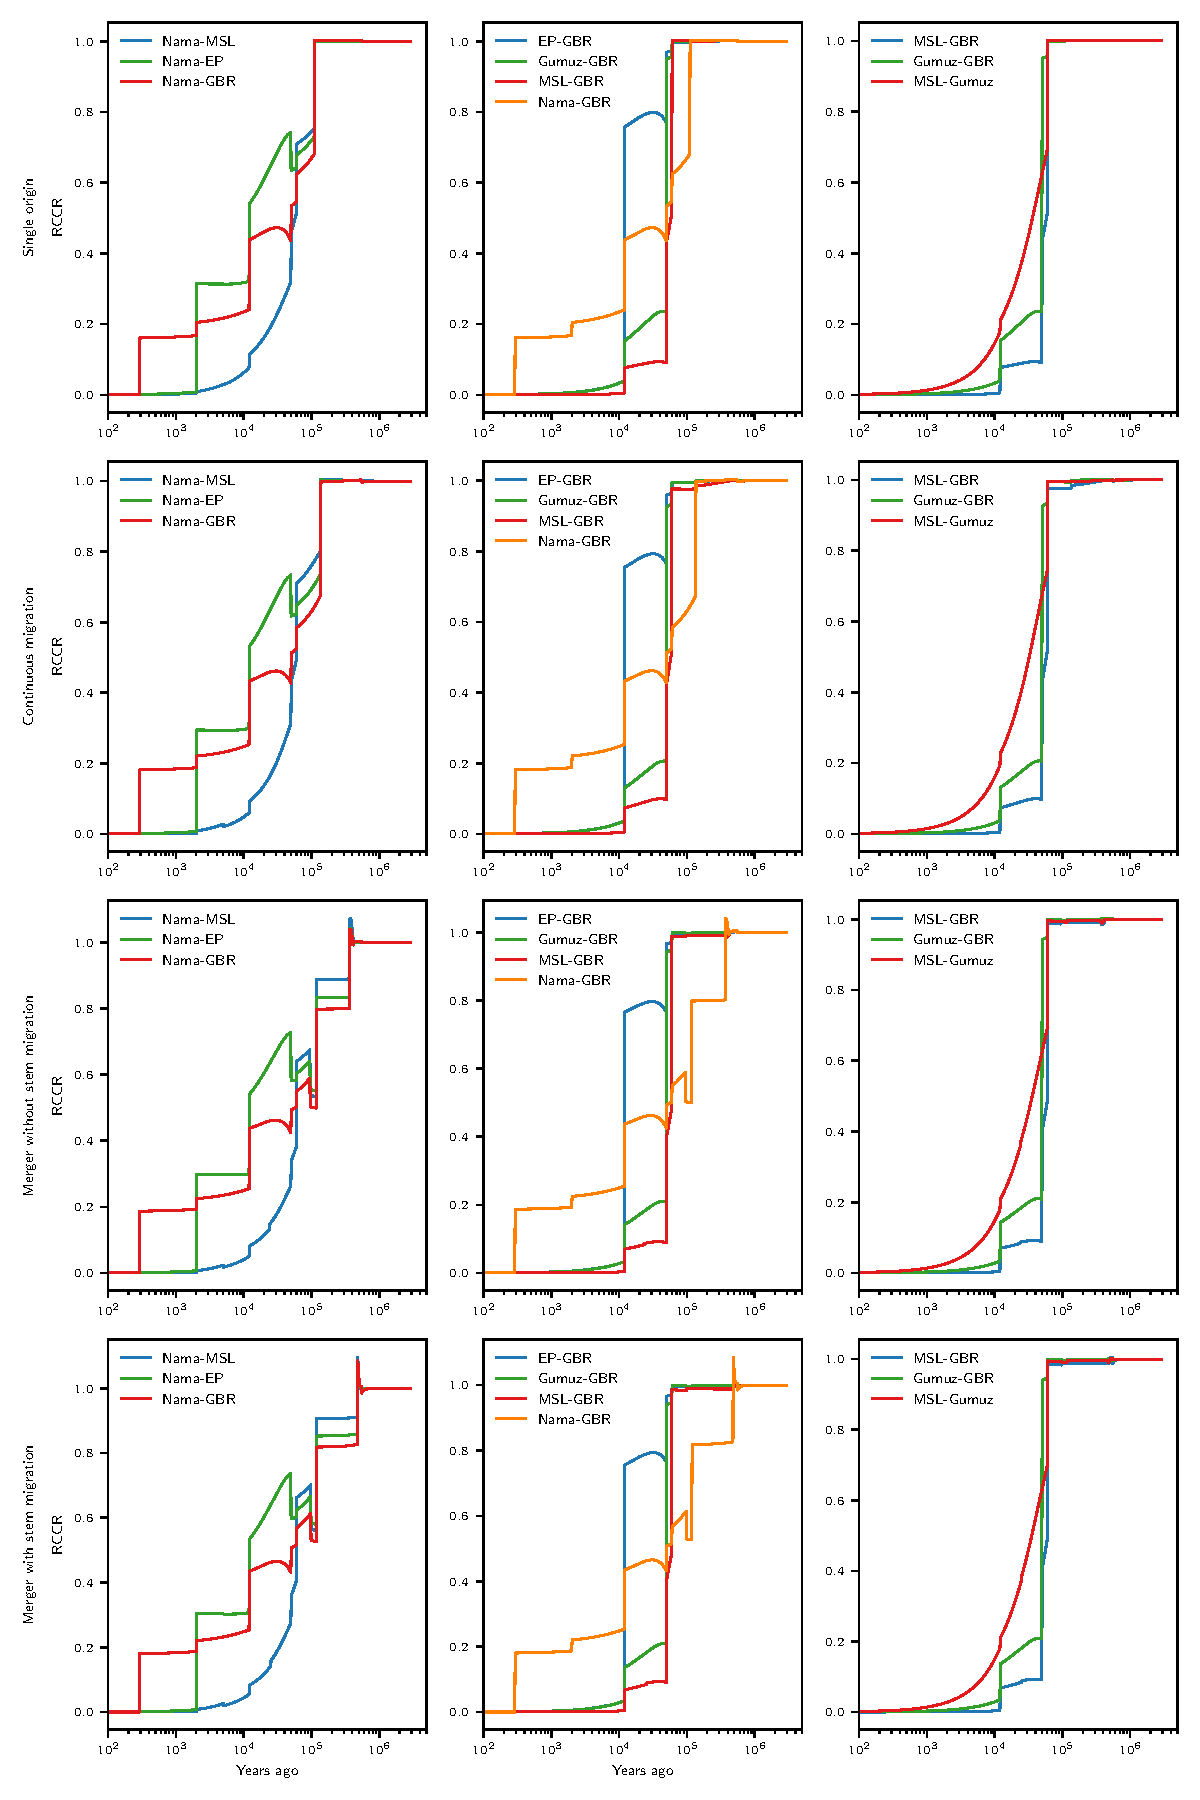
\includegraphics[width=0.75\textwidth]{figures/supp-relate-rccr-model-exp.pdf}
    \caption{
        \textbf{Expected relative cross-coalescence rates from inferred models.}
        Our inferred demographic models allow for exact calculation of expected
        RCCR curves, showing that while the parameterizations of the four models
        are quite different, they each predict very similar RCCR profiles.
    }
    \label{fig:supp-rccr-exp}
\end{figure}

\begin{figure}[ht]
    \centering
    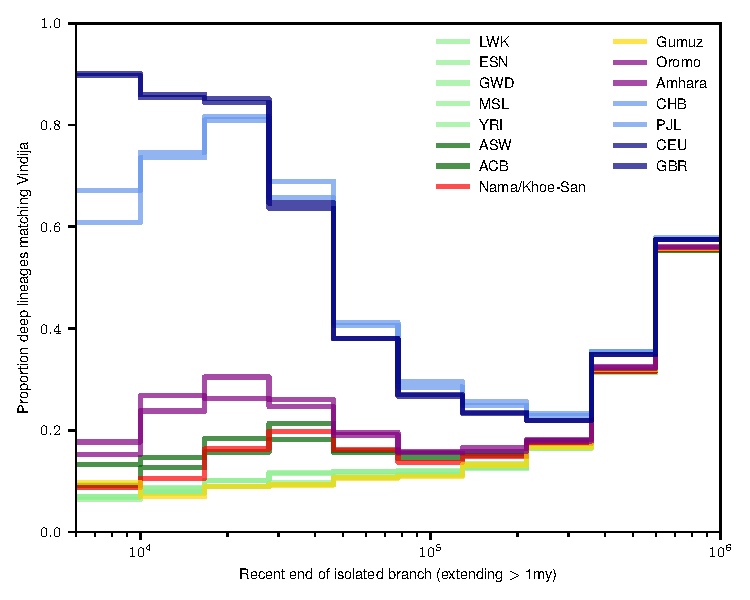
\includegraphics{figures/supp-deep-brances-data}
    \caption{
        \textbf{Neanderthal-matching deep branch distribution from the data.}
        Following the approach of \citet{Speidel2019-nj}, we categorized
        Neanderthal-matching deep branches for each population from
        Relate-inferred gene genealogies. The proportion of deep branches with
        Neandethal affinity is highest for Eurasian populations, as expected,
        and higher for African populations with recent Eurasian ancestry
        (Oromo, Amhara, ACB, ASW, and Nama) than the Gumuz and West African
        populations. 
    }
    \label{fig:supp-deep-branches}
\end{figure}

\begin{figure}[ht]
    \centering
    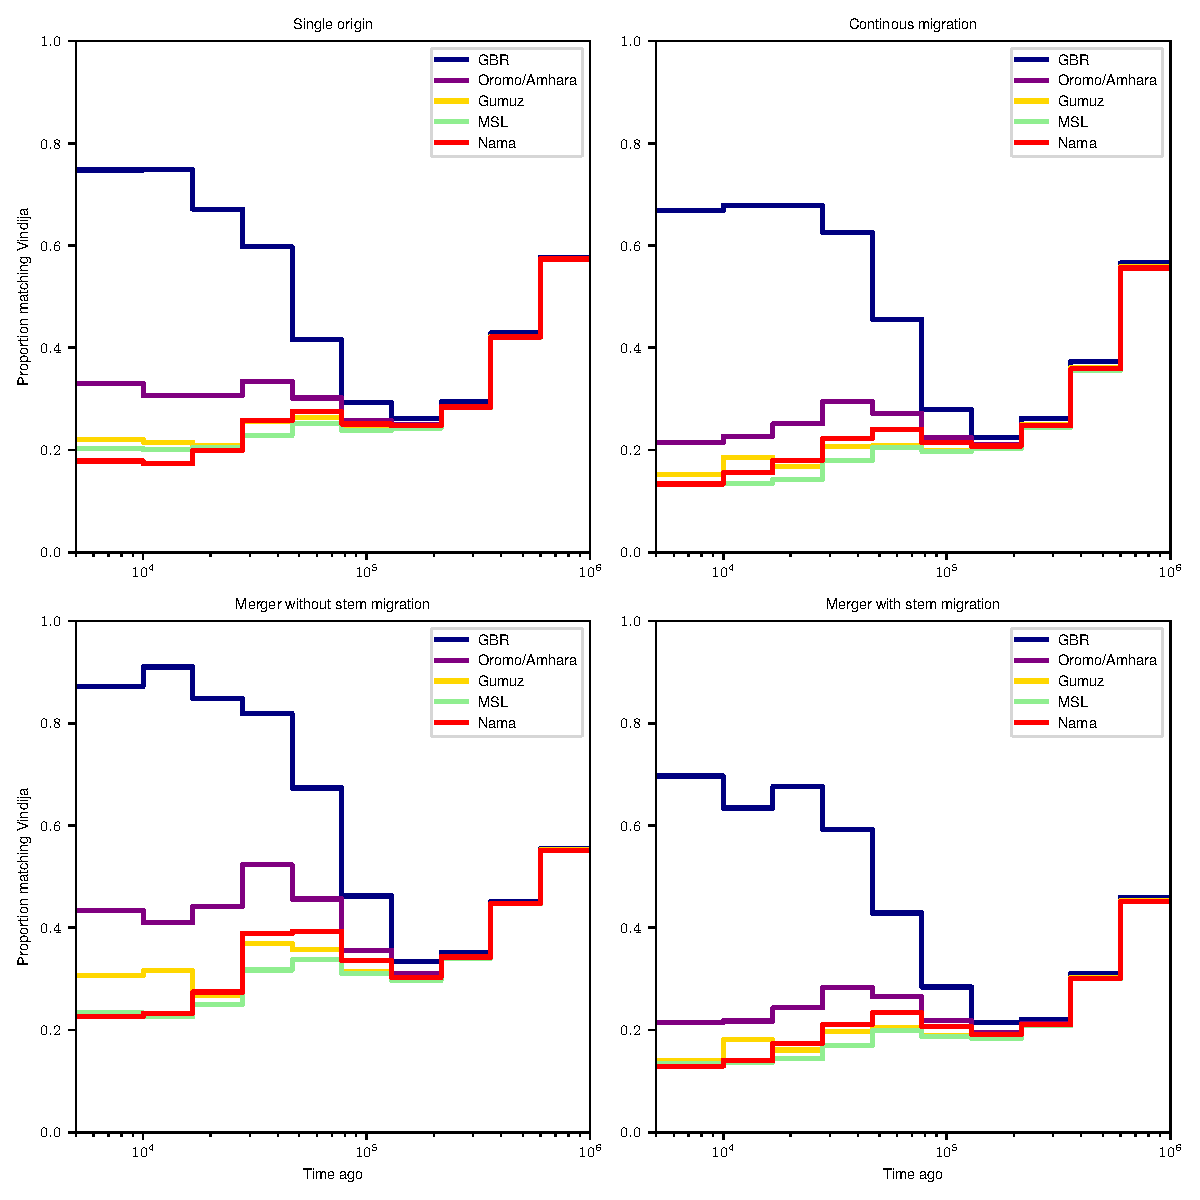
\includegraphics[width=\textwidth]{figures/supp-deep-branches-sim}
    \caption{
        \textbf{Deep branch distribution reinferred from simulated data.} We
        used Relate to reinfer gene genealogies from simulated data under the
        four highlighted models and categorized Neanderthal-matching deep
        branches in the simulated datasets. Each model provided a qualitative
        match to the data (highest proportion of Neanderthal-matching deep
        branches in the British, followed by Amhara/Oromo and Nama). Similar to
        reinferred IIRC and RCCR, no model provided a perfect match to the
        reconstructions using Relate with the data, but the similarities
        between reconstructed genealogies in the simulated data suggest such
        coalescence-rate based curves are underpowered to differentiate between
        plausible models of history.
    }
    \label{fig:supp-deep-branches-sim}
\end{figure}

\begin{figure}[ht]
    \centering
    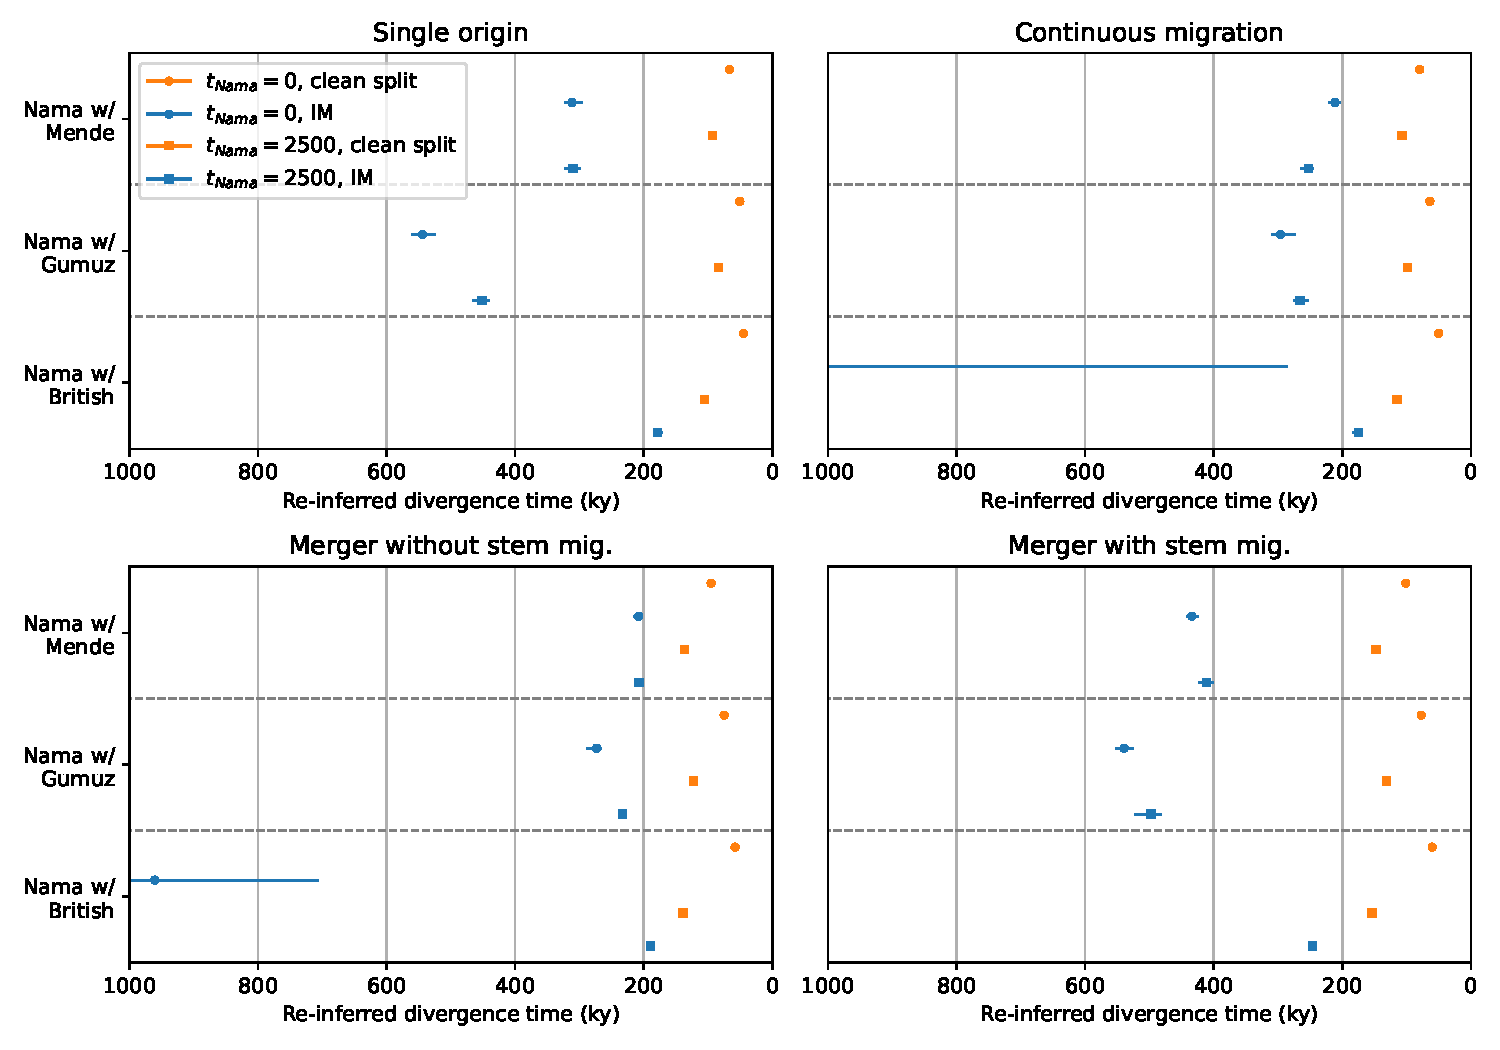
\includegraphics[width=\textwidth]{figures/supp-IM-misspecification}
    \caption{
        \textbf{IM model split times reinferred from simulated data of full
        model.} We simulated 10 diploid individuals under the four highlighted
        models (Sec.~\ref{sec:IM-reinfer}). Using the joint-SFS, we reinferred
        a simpler isolation-with-migration (IM) model for pairs of populations
        including the Nama to explore the effect of model misspecification on
        the earliest inferred divergence times between Khoe-San and other
        populations. We simulated data with Nama individuals sampled at present
        ($t=0$) as well as Nama individuals sampled 2,500 years ago, prior to
        the recent gene flow from East Africans and Europeans. We fit two
        models for each model and population pair: one that allowed for
        migration between the populations (IM), and one that disallowed
        migration (clean split). Despite all original models having recent
        population divergences $\sim120$ka, the reinferred IM models all
        settled on divergence times greater than 200ka and sometimes much
        greater. If the true historical model includes reticulation or
        long-lasting structure, simpler IM models may be severely biased in
        favor of more ancient divergence times.
    }
    \label{fig:supp-IM-misspecification}
\end{figure}

\end{document}
